%
% header.tex
%
\documentclass[%
	pdftex,%              PDFTex verwenden
	a4paper,%             A4 Papier
%	oneside,%             Einseitig
	twoside,%	      Zweiseitig
%	bibtotocnumbered,%    Literaturverzeichnis nummeriert einfügen
%	idxtotoc,%            Index ins Verzeichnis einfügen
%	halfparskip,%         Europäischer Satz mit abstand zwischen Absätzen
%	chapterprefix,%       Kapitel anschreiben als Kapitel
	headsepline,%         Linie nach Kopfzeile
%	footsepline,%         Linie vor Fusszeile
	11pt,%                Größere Schrift, besser lesbar am bildschrim
	openright,%			  Anfang immer auf rechter Seite 
	pointlessnumbers,%	  Nummerierung der Kapitel ohne abschließenden Punkt
%	smallheadings,%		  Kleinere Überschrifen
  headinclude,%
  ]{scrreprt}





%\usepackage{parskip}
%\usepackage{setspace}


\usepackage{url}


%
% Paket für die Indexerstellung.
%
\usepackage{makeidx}


%
% Paket für Übersetzungen ins Deutsche
%
%\usepackage[german, ngerman]{babel}
\usepackage[ngerman]{babel}
 
%
% Pakete um Latin1 Zeichnensätze verwenden zu können und die dazu
% passenden Schriften.
%
\usepackage[utf8]{inputenc}
\usepackage[T1]{fontenc}
%\usepackage{textcomp}
\usepackage{lmodern}  % Schriftart mit deutschen Umlauten

%
% Paket zum Erweitern der Tabelleneigenschaften
%
\usepackage{array}


\newcommand{\todo}[1]{\textbf{\textsc{\textcolor{red}{(TODO: #1)}}}}



%
% Paket um Grafiken einbetten zu können
%
\usepackage[pdftex]{graphicx}
\usepackage{wrapfig}

%
% Spezielle Schrift verwenden.
%
\renewcommand{\encodingdefault}{T1}
%\renewcommand{\familydefault}{pfr}
%\renewcommand{\sfdefault}{pfr}

%
% Spezielle Schrift im Koma-Script setzen.
%
% old:
%\setkomafont{sectioning}{\normalfont\bfseries}
%\setkomafont{llabel}{\normalfont\bfseries}
%\setkomafont{pagehead}{\normalfont\itshape}
%\setkomafont{descriptionlabel}{\normalfont\bfseries}
% new
%\setkomafont{sectioning}{\sffamily\bfseries}
%\setkomafont{captionlabel}{\sffamily\bfseries}
%\setkomafont{captionlabel}{\sffamily}
%\setkomafont{pagehead}{\sffamily\small\itshape}
%\setkomafont{pagehead}{\sffamily\small}
%\setkomafont{descriptionlabel}{\sffamily\bfseries}

%
% Zeilenumbruch bei Bildbeschreibungen.
%
\setcapindent{1em}


\usepackage[size=normalsize]{caption}


%Fussonotennummerierung durch das gesamte Dokument
\usepackage{chngcntr}
\counterwithout{footnote}{chapter}


%
% kopf und fusszeilen
%
%\usepackage[automark]{scrpage2}
%\pagestyle{scrheadings}
%\pagestyle{empty}

\usepackage{fancyhdr} 
\pagestyle{fancy}

\renewcommand{\chaptermark}[1]{\markboth{\MakeUppercase{\thechapter\ #1}}{}}

%
%% Kopf- und Fusszeilen formatieren
\fancypagestyle{normal}{
\fancyhf{}
\renewcommand\headrulewidth{0.4pt}
\fancyhead[RE]{\leftmark}
\fancyhead[LO]{\rightmark}
\fancyhead[RO,LE]{\thepage}
}
% Anfang eines neuen Kapitels etc.
\fancypagestyle{plain}{
\renewcommand\headrulewidth{0.0pt}
\fancyhf{}
\fancyfoot[CO]{\thepage}
}
% Header für das Inhaltsverzeichnis
\fancypagestyle{ihv}{
\fancyhf{}
\renewcommand\headrulewidth{0.4pt}
\fancyhead[RE,LO]{INHALTSVERZEICHNIS}
\fancyhead[RO,LE]{\thepage}
}
% Header für das Abkürzungsverzeichnis
\fancypagestyle{akv}{
\fancyhf{}
\renewcommand\headrulewidth{0.4pt}
\fancyhead[RE,LO]{ABKÜRZUNGSVERZEICHNIS}
\fancyhead[RO,LE]{\thepage}
}
% Header für den Anhang
\fancypagestyle{app}{
\fancyhf{}
\renewcommand\headrulewidth{0.4pt}
\fancyhead[RE,LO]{ANHANG}
\fancyhead[RO,LE]{\thepage}
}
% Header für das Abbildungsverzeichnis
\fancypagestyle{abv}{
\fancyhf{}
\renewcommand\headrulewidth{0.4pt}
\fancyhead[RE,LO]{ABBILDUNGSVERZEICHNIS}
\fancyhead[RO,LE]{\thepage}
}
% Header für das Literaturverzeichnis
\fancypagestyle{bib}{
\fancyhf{}
\renewcommand\headrulewidth{0.4pt}
\fancyhead[RE,LO]{LITERATURVERZEICHNIS}
\fancyhead[RO,LE]{\thepage}
}
% Header für den Index
\fancypagestyle{swv}{
\fancyhf{}
\renewcommand\headrulewidth{0.4pt}
\fancyhead[RE,LO]{INDEX}
\fancyhead[RO,LE]{\thepage}
}
% Header für Listings
\fancypagestyle{lst}{
\fancyhf{}
\renewcommand\headrulewidth{0.4pt}
\fancyhead[RE,LO]{LISTINGS}
\fancyhead[RO,LE]{\thepage}
}

%
% 2-seitiger Druck
%
%\rohead[\pagemark]{\pagemark}
%\rehead[\leftmark]{\leftmark}
%\lohead[\rightmark]{\rightmark}
%\lehead[\pagemark]{\pagemark}
%\ifoot[]{}
%\cfoot[]{}
%\ofoot[]{}
%
% 1-seitiger Druck
%
%\rohead[]{\pagemark}
%\rehead[]{}
%\lohead[]{\leftmark}
%\lehead[]{\pagemark}
%\ifoot[]{}
%\cfoot[]{}
%\ofoot[]{}
%\chead[]{}


%%Zeilenumbruch nach Paragraph
% \usepackage{titlesec}
% \titleformat{\paragraph}%
% {\bf}%
% {\theparagraph}%
% {0.5em}%
% {}


\usepackage{booktabs}
\usepackage{longtable}
\usepackage{multirow}

% \setlength\LTpre{-0.2cm}
% \setlength\LTpost{-1cm}


%%%%%%%%%%%%%%%%%%%%%%%%%%%%%
% Mathematik-Einstellungen

%
% mathematische symbole aus dem AMS Paket.
%
\usepackage{amsmath}
\usepackage{amssymb}
\usepackage{amsthm}

\usepackage{shadethm}

%\usepackage{thmbox}


% Equation Counter
\numberwithin{equation}{section}

% Definitionen
\newtheoremstyle{examplestyle}% name of the style to be used
  {10mm}% measure of space to leave above the theorem. E.g.: 3pt
  {10mm}% measure of space to leave below the theorem. E.g.: 3pt
  {}% name of font to use in the body of the theorem
  {}% measure of space to indent
  {\bfseries}% name of head font
  {\newline}% punctuation between head and body
  {10mm}% space after theorem head
  {}% Manually specify head

\theoremstyle{examplestyle}

\definecolor{shadethmcolor}{rgb}{.95,.95,.95}     % Farbe des Hintergrundes 
%\definecolor{shaderulecolor}{rgb}{0.0,0.0,1.0}   % Farbe des Rahmens
%\setlength{\shadeboxrule}{1pt}   		  % Breite des Rahmens

\newshadetheorem{definition}{Definition}[section]
\newshadetheorem{lemma}{Lemma}[section]
\newshadetheorem{beweis}{Beweis}[section]
\newshadetheorem{voraussetzung}{Voraussetzung}[section]

% Ende Mathematik-Einstellungen
%%%%%%%%%%%%%%%%%%%%%%%%%%%%%



%
% Paket um Textteile drehen zu können
%
\usepackage{rotating}
%\usepackage{lscape}

%
% Package für Farben im PDF
%
\usepackage{color}


%
% Seitenabmessungen
%
\setlength{\topmargin}{0pt}
\setlength{\voffset}{0cm}
\setlength{\textheight}{20.5 cm}
%\setlength{\headsep}{0.7cm}
\setlength{\evensidemargin}{1.15cm}
\setlength{\oddsidemargin}{0.2cm}
\setlength{\marginparwidth}{0.5cm}
\setlength{\textwidth}{14.7cm}
\setlength{\headwidth}{14.7cm}
\setlength{\skip\footins}{15mm}
%\setlength{\footskip}{2cm}


%
% Bis zu welcher Strukturtiefe soll nummeriert werden
%
\setcounter{secnumdepth}{2} 

%
% Hack um doublepages zu löschen
%
\makeatletter
\def\cleardoublepage{\clearpage\thispagestyle{empty}%
  \if@twoside \ifodd\c@page\else
  \hbox{}\newpage%
  \if@twocolumn\hbox{}\newpage\fi\fi\fi}
\makeatother

%
% Paket für Links innerhalb des PDF Dokumentes
%
% \definecolor{LinkColor}{rgb}{0,0,0.5}
\definecolor{LinkColor}{rgb}{0,0,0}
\usepackage[%
	pdftitle={A Rule-Based Approach to the  Semantic Lifting of Model Differences in the context of
	Model Versioning},%
	pdfauthor={Manuel Ohrndorf},%
	pdfcreator={},
	pdfsubject={Bachelorarbeit},
	pdfkeywords={Modelldifferenzen},
	plainpages=false,
	pdfpagelabels,
	bookmarksnumbered=true,
	bookmarksopen=true,
	pdfpagemode=UseOutlines]
	{hyperref}
\hypersetup{colorlinks=true,%
	linkcolor=LinkColor,%
	citecolor=LinkColor,%
	filecolor=LinkColor,%
	menucolor=LinkColor,%
	pagecolor=LinkColor,%
	urlcolor=LinkColor}

%
% Paket um Listings sauber zu formatieren.
%
\usepackage{listings}
\lstloadlanguages{TeX}

%
% Neue Sprachdialekte
%
%
% Pseudocode
%
\lstdefinelanguage{pseudo}{
	keywords={in, if, endif, else, for , endfor, function, return, break, true, false, when, each, new, boolean},
	sensitive=true,
	comment=[l]{//}
}

%              
% WORKAROUND, damit lstlistoflistings funktioniert:
% Quelle: http://www.komascript.de/node/477
%
\makeatletter% --> De-TeX-FAQ
\renewcommand*{\lstlistoflistings}{%
  \begingroup
    \if@twocolumn
      \@restonecoltrue\onecolumn
    \else
      \@restonecolfalse
    \fi
    \lol@heading
    \setlength{\parskip}{\z@}%
    \setlength{\parindent}{\z@}%
    \setlength{\parfillskip}{\z@ \@plus 1fil}%
    \@starttoc{lol}%
    \if@restonecol\twocolumn\fi
  \endgroup
}
\makeatother% --> \makeatletter

%
% Abkürzungsverzeichnis
%
\usepackage{nomencl}
% Befehl umbenennen in abk
\let\abk\nomenclature
% Deutsche Überschrift
\renewcommand{\nomname}{Abkürzungsverzeichnis}
% Punkte zw. Abkürzung und Erklärung
\setlength{\nomlabelwidth}{.20\hsize}
\renewcommand{\nomlabel}[1]{#1 \dotfill}
% Zeilenabstände verkleinern
\setlength{\nomitemsep}{-\parsep}
\makenomenclature

%
%Für Gedanken an der Seite => mit der letzten Zeile wird das wieder auskommentiert
%
\newcommand{\marginlabel}[1]{\mbox{}\marginpar{\raggedleft\hspace{0pt}#1}}
\newcommand{\Gedanke}[1]{\marginlabel{#1}}
%\renewcommand{\Gedanke}[1]{}           % outcomment this to get Gedanken!

%
% ---------------------------------------------------------------------------
% Listing Definationen für Code
%
% 



\definecolor{lbcolor}{rgb}{0.95,0.95,0.95}
\definecolor{commentcolor}{rgb}{0.4,0.4,0.4}
\lstset{language=pseudo,
	numbers=left,
	stepnumber=1,
	numbersep=5pt,
	numberstyle=\tiny,
%	breaklines=true,
% 	breakautoindent=true,
% 	postbreak=\space,
	tabsize=2,
	basicstyle=\small,
	commentstyle=\color{commentcolor}\itshape,
	stringstyle=\ttfamily,
	keywordstyle=\color{black}\bfseries,
	showspaces=false,
	showstringspaces=false,
	extendedchars=true,
	backgroundcolor=\color{lbcolor}}
%
% ---------------------------------------------------------------------------
%

%
% Zeilenabstand
%
\renewcommand{\baselinestretch}{1.2}

%% Schusterjungen und Hurenkinder vermeiden
%\clubpenalty = 10000 %Schusterjunge
%\widowpenalty = 10000 %Hurenkind


% Wird statt siehe bspw. die Abk. s. bevorzugt:
\renewcommand{\seename}{s.}

%
% Löst das Problem der franz. Anführungszeichen über verbatim-Umgebung
%
%\newcommand {\franzL} {\begin{verbatim}<<\end{verbatim}}
%\newcommand {\franzR} {\begin{verbatim}>>\end{verbatim}}
%\newcommand {\frq} {\begin{verbatim}<\end{verbatim}}
%\newcommand {\flq} {\begin{verbatim}<\end{verbatim}}

%
% Neue Umgebungen
% ---------------------------------------------------------------------------

\newenvironment{ListChanges}%
	{\begin{list}{$\diamondsuit$}{}}%
	{\end{list}}

%
% Index erzeugen
%
\makeindex

%
% EOF
%



%\usepackage{tabularx} 
%\usepackage{amsmath} 
% 
%\usepackage{multicol} 
%\usepackage{float} 
%\usepackage{amssymb} 
%
%\usepackage{pifont}  
%\include{codestyle} 

 
\begin{document}

%\input{misc/glossary}

%
% Counter für Teile des Dokumentes
%
%\newcounter{Dokumentteil}
%\addtocounter{Dokumentteil}{1}


\pagenumbering{roman}

\pagestyle{empty}
\begin{titlepage}
\ifpdf\pdfbookmark{Titlepage}{title}\fi	% Zum PDF Inhaltsverzeichnis hinzufügen
\begin{center}
  \includegraphics[scale=0.20]{logoSiegen} \\
  \vspace{3cm}
  \Large{\textbf{Master's Thesis}}
  \\
  \vspace{1cm}
  \huge{\textbf{ Integration of UML Profiles into the SiDiff and SiLift tools}}
  \\
  \medskip
  \Large{\textbf{Based on a SysML case study}}
  \\
  \vspace{2cm}
  \Large{Dennis Reuling} \\
  \vspace{4cm}
\textsf{
    \begin{large}
    \begin{tabular}{ll}
      Faculty: & Faculty of Science and Technology \\
      Department: & Electrical Engineering and Computer Science \\
      Institute: & Software Engineering Group\\
      Reviewers: & Prof. Dr. Udo Kelter, Dipl. Inf. Timo Kehrer \\
      Date: & \today
    \end{tabular}
  \end{large}
  }
\end{center}
\end{titlepage}

\cleardoublepage



\textbf{Kurzfassung:}\hspace{0.3cm} Im Zentrum des \textit{Model-Driven Software Development} (MDSD)
stehen Modelle, welche häufig durch Teams entwickelt werden. Um in einem Team mit Modellen zu
arbeiten, werden Versionsverwaltungswerkzeuge benötigt. Eine Hauptaufgabe dieser Werkzeuge ist das
Vergleichen von verschiedenen Versionen oder Varianten eines Modells. Um zwei Modelle miteinander
zu vergleichen wird eine Differenz zwischen den beiden Modellen durch ein spezielles
Differenzwerkzeug berechnet. Da es eine Vielzahl von verschiedenen Modelltypen gibt, müssen die
Differenzwerkzeuge generisch arbeiten um mit allen Modelltypen umgehen zu können. Dadurch entsteht
allerdings das Problem, dass die Differenz zwischen zwei Modell Versionen nur auf Basis der internen
Repräsentation der Modelle angegeben werden kann. Die Differenzen auf Basis der internen Darstellung
werden hier als  low-level Änderungen bezeichnet. Solche low-level Änderungen sind aber für
Entwickler die nur die externe Repräsentation der Modelle kennen schwer zu lesen. Diese Arbeit setzt
sich damit auseinander die Lesbarkeit der Differenzen zu verbessern, indem den low-level Änderungen
wieder bestimmte Editieroperationen zugeordnet werden.
% Die Änderungen einer Editieroperation werden durch eine s.g. Editierregel vorgegeben. Das Auslesen
% der Editieroperation aus der Differenz wird durch die s.g. Erkennungsregeln erledigt. Eine
% Erkennungsregel sucht in der Differenz nach einem Muster von low-level Änderungen die zu der
% entsprechenden Editierregel passen. Anschließend werden die low-level Änderungen zu einer
% Editieroperation in einem s.g. Semantic-Change-Set gruppiert.
Dieser Prozess wird hier als Semantic-Lifting bezeichnet.

\vspace{1cm}

\textbf{Abstract:} \hspace{0.3cm} Models are in the center of \textit{Model-Driven Software
Development} (MDSD) and they are often developed in teams. To comply with the task of sharing a
model among team members we need special version management tools. One main task of a version
management tool is the comparison of different model versions. We also need special model difference
tools to calculate the changes between the two models. The algorithms of the difference tools have
to deal with many different model types. Instead of developing an individual algorithm for each
model type, the difference tools have to be generic. One problem of a generic difference algorithm
is that it has to compare the models based on their internal representation. Thus, difference tools
initially derive low-level changes from the internal representation of a model. But the low-level
changes are often incomprehensible for normal tool users, who usually prefer model changes to be
explained in terms of edit operations that are available from a user's point of view. So the primary
goal here is to increase the readability of the difference by lifting the low-level changes to the
level of user edit operations. We will call this process Semantic-Lifting.

\clearpage

\setcounter{page}{0} 


\pagestyle{ihv}
\tableofcontents
\cleardoublepage


\pagestyle{normal}




\pagenumbering{arabic}

%
% ---------------------------------------------------------------------------
%


% Textabschnitte

\chapter{Einleitung}

Sowohl unser Geschäfts- als auch unser Alltagsleben sind heutzutage durch Softwaresysteme geprägt.
Dabei werden sowohl aus Benutzersicht als auch aus technischer Sicht hohe Anforderungen an die
verwendete Software gestellt. Eine Software soll gut bedienbar, zuverlässig, sicher, vernetzbar,
anpassbar und dabei auch möglichst günstig sein. Um diesen Anforderungen gerecht zu werden, werden
die Software Projekte auf technischer Seite zum einen immer komplexer und größer, zum anderen muss
ein solches Projekt häufig über Jahre oder Jahrzehnte hinweg gepflegt und gewartet werden. Im Laufe
dieser Zeit kann es passieren, dass sich gewisse Anforderungen an das Projekt ändern oder dass die
Software auf eine neu entwickelte Technologie übertragen werden soll. Nicht zuletzt spielen auch die
Kosten, die in eine solche Entwicklung einfließen eine entscheidende Rolle. Daher werden immer neu
Methoden benötigt, um die effektive Entwicklung und Wartung eines Softwaresystems zu ermöglichen.

% \begin{quote}
% "`The myth of the standalone application, never needing repair, never needing
% integration, with data models inviolate and secret, died a long and painful death
% through the end of the Twentieth Century. Despite the sure knowledge that every
% application ever built must be built to last, to be integrated, to be updated, most
% software developers ignored these facts and built only to the specification in front of
% them. Assumptions not in evidence–'this application will only be needed for the next
% few years,` [\ldots]"' \cite{MDA} (S.5)
% \end{quote}

% Eine fehlerhafte Annahme, die in der Vergangenheit oft getroffen wurde, ist die, dass eine Software
% nur ein paar Jahre gebraucht wird und anschließend keine Weiterentwicklung und Wartung mehr
% stattfindet. Würden wir unter der gleichen Annahme Gebäude bauen, dann wäre es uns unmöglich diese
% zu verändern oder auch einfach nur umzudekorieren, um sie an neue Gegebenheit anzupassen und im
% schlimmsten Fall würde sie auf Dauer einfach in sich zusammenfallen. Während dies neue Arbeit für
% Bauarbeiter schafft, sind diese Umstände hingegen für die Menschen, die in diesen Gebäuden leben und
% arbeiten absolut inakzeptabel. Deshalb gibt es eigentlich nur sehr wenig Ausreden dafür eine
% Software zu entwickeln, ohne vorher sorgfältige Planungsarbeiten durchzuführen. Die Planungsarbeiten
% helfen nicht nur dabei ein Softwaresystem einfach zu entwickeln, zu integrieren und zu warten,
% sondern sie geben uns auch die Möglichkeit einige Teile des Systems automatisch zu erzeugen. So, als
% ob eine Maschine sofort aus dem Modell eines Architekten die Grundkonstruktion eines Gebäudes
% erstellten könnte. Mehr noch, wenn wir verschiedene Konstruktionen verbinden wollen, können wir
% automatisch Brücken basierend auf den vorliegenden Modellen generieren und wenn ein neuer
% feuerfester Stahltyp entwickelt wurde, dann können wir alle Konstruktionen auf dieser Grundlage
% einfach erneut generieren. \cite{MDA} (S.5-6)

% The myth of the standalone application, never needing repair, never needing
% integration, with data models inviolate and secret, died a long and painful death
% through the end of the Twentieth Century. Despite the sure knowledge that every
% application ever built must be built to last, to be integrated, to be updated, most
% software developers ignored these facts and built only to the specification in front of
% them. Assumptions not in evidence–“this application will only be needed for the next
% few years,” a particular favorite–wreaked havoc in the business world as the clock
% ticked over to the year 2000. Nevertheless, most software continues to be written
% ignoring the realities of constantly shifting infrastructure, constantly changing
% requirements, and most importantly, a new “hot technology” trumpeted on the covers
% of every IT trade journal every 18 months.

% After all, if we built buildings the way we built software, we would be unable to
% connect them, change them or even redecorate them easily to fit new uses; and worse,
% they would constantly be falling down. While this might generate new income for
% construction workers, it might not be acceptable to those who live and work in those
% buildings.

% In fact, we have very little excuse to build software without first doing careful design
% work; design not only leads to systems that are easier to develop, integrate and
% maintain–but also because we have the ability to automate at least some of the
% construction. Imagine if the construction worker could take his blueprint, crank it
% through a machine, and have the foundation of the building simply appear. Not likely
% outside the Jetsons’ world, but an everyday occurrence in the software world. We can
% take models, defined in standards like OMG’s own UML, MOF and CWM, and
% automate the construction of data storage and application foundations. Even better,
% when we need to connect these “buildings” to each other we can automate the
% generation of bridges and translators based on the defining models; and when a new,
% more fire-resistant type of steel is invented, we can regenerate for the new
% infrastructure.

Ein Konzept, welches in der Praxis immer mehr an Bedeutung gewinnt, ist das \textit{Model-Driven
Software Development} (MDSD) \cite{MDA}, \cite{MDSD}, \cite{GPR06}. Die Philosophie hinter diesem
Softwareentwicklungskonzept ist es,
% Eben diese Philosophie steckt hinter dem Softwareentwicklungskonzept des \textit{Model-Driven
% Software Development} (MDSD),
möglichst viele Teile der Softwareherstellung zu automatisieren. Als Grundlage hierfür werden
hinreichend formale und zugleich abstrakte Modelle verwendet, aus denen dann verschiedene Artefakte
des Systems abgeleitet werden. Modelle werden dabei vorzugsweise als Diagramme angelegt, da komplexe
Strukturen visuell so besser überblickt werden können. Die abgeleiteten Artefakte können zum einen
ausführbare Programmteile in einer bestimmten Zielsprache wie z.B. Java oder C\# sein, zum anderen
können aber auch Konfigurationsdateien, Datenbankskripte, Testfälle oder Dokumentationsdateien aus
den Modellen automatisch abgeleitet werden, während  dieser Prozess in der klassischen Software
Entwicklung eine manuelle Tätigkeit ist. Daher nehmen Modelle in MDSD ein zentrale Stellung im
gesamten Entwicklungsprozess einer Software ein. \cite{MDSD} (S.11 - 13)

\begin{quote}
"`Das bedeutet auch, dass Modelle und einzelne Modellelemente z.B. bezüglich Versionierung genauso
zu behandeln sind wie Quelltext. Verteilte Teams müssen also in der Lage sein, Modelle aus einem
Versionsverwaltungssystem auszuchecken, einzelne Modellelemente zu bearbeiten, mit früheren
Versionen zu vergleichen, konkurrierende Modifikationen aufzulösen und den neuen Stand wieder in das
Versionsverwaltungssystem einzuchecken."' \cite{MDSD} (S.12)
\end{quote}

Um verschiedene Versionen von Modellen zu vergleichen und um die Unterschiede zwischen den Versionen
anzuzeigen, werden s.g. Differenzwerkzeuge benötigt. Differenzwerkzeuge, mit denen normalerweise
Quelltexte verglichen werden, sind für strukturierte Modelle nicht zu gebrauchen \cite{LE09}, da
diese auf Basis ihrer Graphrepräsentation verglichen werden müssen. Viele verfügbare
Differenzwerkzeuge arbeiten generisch, so dass sie für verschiedene Modelltypen eingesetzt werden
können. Ein Nachteil, der daraus resultiert, ist, dass die Modelle anhand ihrer internen
Repräsentation verglichen werden müssen. Diese interne Repräsentation unterscheidet sich aber oft
signifikant von der externen Darstellung der Modelle. Ein Entwickler, der mit einem bestimmten
Modelltyp arbeitet, kennt vielleicht die interne Repräsentation gar nicht. Es wäre also am besten,
wenn die Differenz zwischen zwei Modellen als Abfolge von Editierschritten auf Basis der externen
Darstellung angezeigt würde. \cite{KeKT2011ASE} (S.1)

\begin{figure}[htb]
  \centering
  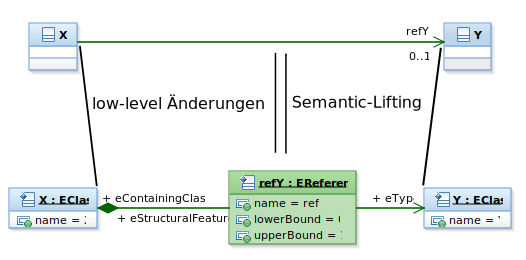
\includegraphics[width=1.0\textwidth]{images/semantic_lifting.png}
  \caption{Semantic-Lifting}
  \label{fig:semantic_lifting}
\end{figure}

Abbildung \ref{fig:semantic_lifting} demonstriert dies anhand des Einfügens einer Referenz zwischen
zwei Klassen eines Ecore Modells (Abbildung \ref{fig:ecore_metamodel}). Wie man sieht wird dazu in
der internen Darstellung eine neue Klasse angelegt, die diese Referenz repräsentiert. Sowohl der
Name als auch die Multiplizitäten der Referenzen werden als Attribute in dieser Klasse gespeichert.
Zusätzlich werden noch mehrere Referenzen benötigt, welche Quelle und Ziel der eingefügten Referenz
festlegen. Eben diese s.g. \textbf{low-level Änderungen} werden durch das Differenzwerkzeug erkannt
und angezeigt. Die Frage ist nun, ob es möglich ist nur anhand der low-level Änderungen zu erkennen,
welche Editieroperation auf das Modell angewendet wurde, um dem Benutzer so eine Differenz auf Basis
der externen Repräsentation anzuzeigen.

Das Konzept "`A Rule-Based Approach to the Semantic Lifting of Model Differences in the Context of
Model Versioning"' \cite{KeKT2011ASE} beschäftigt sich mit genau dieser Problematik. Hier wird ein
Algorithmus beschrieben, der einer beliebigen Anzahl von low-level Änderungen wieder die
entsprechenden Editieroperationen zuordnen kann. Dazu werden Editierregeln verwendet, welche eine
Editieroperation beschreiben. Die Editierregeln werden dann dazu benutzt, um das der Editieroperation
entsprechende Muster von low-level Änderungen wieder zu erkennen.  Dieser Prozess wird in Anlehnung
an das Konzept im Folgenden als \textbf{Semantic-Lifting} bezeichnet. 

Diese Arbeit beschreibt die praktische Untersuchung, Implementierung und die daraus resultierenden
Ergebnisse des Semantic-Liftings. Dazu werden in Kapitel \ref{grundlagen} zunächst die wichtigsten
Technologien für dieses Projekt besprochen. Kapitel \ref{diffPipe} gibt einen Überblick über
den im Folgenden beschriebenen Algorithmus. Hierzu wird in den Kapiteln \ref{editierregeln},
\ref{generierung} und \ref{verwaltung} die Erstellung von Editierregeln und die Generierung von
daraus resultierenden Mustern zur Erkennung der Editeroperationen erläutert. In den Kapiteln
\ref{resource_sets}, \ref{recognition}, \ref{post_processing}, \ref{sequential} und
\ref{benutzer}, wird dann dargelegt, wie mit Hilfe dieser Erkennungsmuster, das eigentlich
Semantic-Lifting durchgeführt wird. In Kapitel \ref{evaluierung} und \ref{schlussfolgerung} werden
zum Schluss die Ergebnisse des Semantic-Liftings ausgewertet.

\chapter{Grundlagen}
\label{grundlagen}

Im Folgenden werden die beiden wichtigsten Technologien vorgestellt, die als Grundlage für diese
Arbeit verwendet wurden. Zum einen das Eclipse Modeling Framework, welches die Umgebung für die
gesamte Implementierung darstellt und zum anderen die Modell Transformationssprache Henshin als
wichtigste Technolgie zur Umsetzung des Semantic-Liftings.

\section{Eclipse Modeling Framework}

Das Eclipse Modeling Framework (EMF) ist, wie der Name schon sagt, ein auf Eclipse basierendes
Framework zur Generierung von Quelltext aus Modellen. EMF bildet dabei eine Brücke zwischen
verschiedenen Modellierungsansätzen. Als Eingabe für EMF können z.B. UML-Diagramme, XML-Schemata
oder spezielle Java Interfaces dienen. Damit EMF diese Daten weiter verarbeiten kann, wird dann aus
jedem Eingabemodell ein entsprechendes Modell im EMF eigenen Modelltyp Ecore erzeugt. EMF bietet
aber auch Editoren, in denen Ecore Modelle direkt erzeugt und bearbeitet werden können. Ecore ist
ein s.g. plattformunabhängiges  Metamodell (\textit {engl. platform independent model (PIM)}), d.h.
durch Ecore wird noch nicht festgelegt, für welche Zielplattform später Quelltext generiert werden
soll und wie die konkrete Implementierung des Modells aussehen wird. Eine etwas vereinfachte Form
des Ecore Metamodell ist in Abbildung \ref{fig:ecore_metamodel} zu sehen. Ecore ist eine Implementierung
des EMOF (\textit{Essential Meta Object Facility} \cite{MOF}) Metamodells. EMOF beschreibt einen
Ausschnitt des Metamodells der UML 2.0. Die in Ecore formulierten Modelle dienen nur dazu, die
Datenstrukturen eines Programms zu beschreiben. In der gesamten UML gibt es hingegen aber auch
Modelle, um das Verhalten einer Software zu beschreiben. So wie EMOF ist Ecore ein Modell, welches
sich selbst definiert, d.h. das Metamodell von Ecore ist selbst ein Ecore Modell. Man spricht dann
auch von einem selbstreferentiellen Metamodell.

\begin{figure}[htb]
  \centering
  \includegraphics[scale=0.18]{images/emf_toolset.png}
  \caption{"`EMF Toolset from 30.000 Feet"' \cite{EMFCon} (S.7)}
  \label{fig:emf_toolset}
\end{figure}

Wie in Abbildung \ref{fig:emf_toolset} dargestellt, wird neben dem Ecore Modell zur
Quelltext-Gene"-rie"-rung noch ein s.g. Generator Modell (\textit{GenModel}) benötigt. Das Generator
Modell wird weitestgehend automatisch erzeugt und erweitert das plattformunabhängige Ecore Modell um
plattformspezifische Informationen. Das Generator Modell kann vom Benutzer angepasst werden und
steuert direkt die Quelltext Ausgabe des darunter liegenden Generators. Innerhalb des Generators
findet nun eine s.g. Modell-zu-Text Transformation statt, d.h. aus dem Generator Modell wird nun der
eigentliche Quelltext generiert. Dazu werden Java Emitter Templates (JET) verwendet, diese enthalten
Textmuster die vorgeben wie die Modell-Elemente zu transformieren sind. Die Zielsprache von EMF ist
grundsätzlich Java. Theoretisch kann JET aber auch verwendet werden, um einen Generator zu
schreiben, der aus dem plattformunabhängigen Ecore Modell z.B. SQL oder C\# Quelltext erzeugt. In
Abbildung \ref{fig:emf_toolset} sind die drei wichtigsten Pakete zu sehen, die generiert werden
können:

\begin{itemize}
  \item \textbf{EMF.model:} Der hier erzeugte Java Quelltext ist ein s.g. plattformspezifisches
  Modell (\textit{engl. platform specific model (PSM)}). Dieses stellt die Implementierung des zuvor
  in Ecore beschriebenen plattformunabhängigen Modells dar. Der Java Quelltext ist in der Regel
  sofort ausführbar, um als Datenmodell für eine drauf aufbauende Applikation eingesetzt zu werden.
  An gegebenen Stellen kann bzw. muss der Entwickler dann noch eigenen Code einfügen.
  
  \item \textbf{EMF.edit:} Dieses Paket stellt eine Zugriffsschicht zwischen Modell und
  Modell-Editor dar. Zum einen wird durch die Zugriffsschicht festgelegt, welche Befehle der Editor
  auf dem Modell ausführen darf, zum anderen werden die Daten des Modells für den Editor ggf. in
  passender Form aufbereitet. Je nach benötigter Funktionalität kann die Zugriffsschicht dann noch
  an die Gegebenheiten des Editors angepasst werden.
  
  \item \textbf{EMF.editor:} Hier stellt EMF einen einfachen baumbasierten Editor zum Erstellen und
  Bearbeiten von Modell Instanzen zur Verfügung. Der Editor wird häufig noch manuell angepasst oder
  auch vollständig ersetzt.
\end{itemize}
EMF bietet noch viele weitere Unterstützungen um Modelle zur Laufzeit zu verändern, diese zu
Validieren oder die Daten auf Basis von XML zu Serialisieren. Eine ausführliche Einführung in die
umfangreichen Funktionalitäten von EMF ist in \cite{SBPM2009}, \cite{EMFCon} und unter \cite{EMF} zu
finden.

\begin{figure}[h!]
  \centering
  \includegraphics[scale=0.7]{images/ecore_metamodel.png}
  \caption{Ecore Metamodell (vereinfacht)}
  \label{fig:ecore_metamodel}
\end{figure}

% \newpage

\section{Henshin}

Der Name "`Henshin"' bedeutet Transformation auf Japanisch. Henshin ist eine auf EMF
basierende \textit{in-place} Transformationssprache für Ecore Modelle. Als \textit{in-place} werden
Transformationssprachen bezeichnet, die Änderungen direkt (zur Laufzeit) am Modell durchführen. Im
Gegensatz dazu würde eine \textit{out-place} Transformationssprache das Ursprungsmodell nicht
verändern und eine neue Instanz des Modells mit den durchgeführten Änderungen erzeugen.
Grundsätzlich kann Henshin aber ebenfalls als \textit{out-place} Transformationssystem verwendet
werden, indem man ein Modell in Henshin lädt, die Transformation durchführt und das Modell wieder an
einem anderen Ort abspeichert.

Weitere Informationen über Henshin sind in \cite{Arendt2010}, \cite{BES10} und unter
\cite{HENSHIN} zu finden. Die folgenden Abschnitte geben einen kurzen Überblick über die Henshin
Funktionalitäten.

\subsection{Regeln}

Henshin ist ein Graphersetzungssystem, dieses Konzept beruht auf der Graphentheorie. Ein Graph ist
in Henshin typisiert und besteht aus Knoten, gerichteten Kanten und Attributen. Eine Transformation
wird durch eine Regel angegeben. Diese Regel besteht aus einer linken (\textit{Left-Hand Site}
(LHS)) und einer rechten Seite (\textit{Right-Hand Site} (RHS)). Beide Seiten der Regel sind
Graphen. Der Grundgedanke bei Graph-Transformationsregeln ist ähnlich wie bei Produktionsregeln von
Chomsky-Grammatiken für Texte, es wird innerhalb des s.g. Arbeitsgraphen ein Bild gesucht, welches
der linken Seite entspricht. Man spricht auch von einer Abbildung (\textit{engl. Match}) oder im
Sinne der Graphentheorie von einem Graphmorphismus der linken Seite auf den Arbeitsgraphen. Wurde
eine solche Abbildung gefunden, dann wird diese durch die rechte Seite ersetzt.  Konnte die
Transformation korrekt durchgeführt werden, dann wird die Regel als anwendbar bezeichnet.
Zusätzlich muss noch der Schnitt von LHS und RHS angegeben werden. Dazu müssen in Henshin Mappings
zwischen allen LHS und RHS Knoten angelegt werden, die den gleichen Knoten repräsentieren. Der
Schnitt zwischen LHS und RHS ist genau der Teil der Abbildung, der beim Ausführen der Regel bewahrt
(also nicht verändert) wird. Alle Teile der linken Seite, die nicht im Schnitt enthalten sind,
werden also aus dem Arbeitsgraphen entfernt. Alle Teile der rechten Seite, die nicht im Schnitt
enthalten sind, werden im Gegensatz dazu neu in den Arbeitsgraphen eingefügt.

Um die Abbildungen einer Regel einzuschränken, können zusätzlich noch s.g. \textit{negativ
application conditions} (NAC) formuliert werden. Eine NAC ist ebenfalls ein Graph. Allerdings darf
sich dieser NAC Graph nicht auf den Arbeitsgraphen abbilden lassen, damit die Regel angewendet
werden darf. Mehrere NACs können über eine \texttt{AND} Formel logisch miteinander verbunden werden.

Für jeden Knoten können auch, entsprechend seinem Typ, Attribute angelegt werden. Jedes Attribut hat
einen bestimmten Wert. Der Wert eines Attributs kann entweder ein primitiver Wert sein oder ein
\textit{JavaScript} Ausdruck. Innerhalb des Ausdrucks können Parameter verwendet werden. Diese
werden einfach mit dem entsprechenden Namen für die Regel angelegt. Ein Parameter kann entweder beim
Aufrufen von außen an die Regel übergeben werden oder er wird beim Abbilden der linken
Seite mit einem Wert aus dem entsprechenden Objekt des Arbeitsgraphen initialisiert. Dazu muss es
mindestens ein Henshin Attribut auf der linken Seite der Regel geben, welches nur den Parameter
als Wert besitzt. Der Ausdruck wird dann durch die Rhino Script-Engine \cite{RIHNO}  verarbeitet und
ausgewertet.

Wird ein Attribut auf der rechten Seite der Regel für einen Knoten angelegt, so wird der Wert des
Attributs in das Objekt des Arbeitsgraphen geschrieben, auf welches der Knoten abgebildet wurde.
Wird ein Attribut hingegen auf der linken Seite angelegt, dann muss sich der Wert ebenfalls auf den
Arbeitsgraphen abbilden lassen, sofern das Attribut nicht wie zuvor beschrieben zur Initialisierung
eines Parameters verwendet wurde.

\begin{figure}[htb]
  \centering
  \includegraphics[scale=0.7]{images/henshin_metamodel.png}
  \caption{Henshin Metamodell für Regeln}
  \label{fig:henshin_metamodel}
\end{figure}

Das Henshin Metamodell, über welches die Regeln intern dargestellt werden, ist in Abbildung
\ref{fig:henshin_metamodel} zu sehen. Das Modell basiert auf Ecore und somit können beliebige
Modelle transformiert werden, die ebenfalls auf Ecore basieren.

\subsection{Units}

Mehrere Regeln werden in Henshin in Transforamtionssystemen zusammengefasst. Um den Ablauf einer
Transformation mit mehreren Regeln zu steuern, werden s.g. Units verwendet. Manche Units können auch
ineinander verschachtelt werden (siehe Abbildung \ref{fig:henshin_metamodel_units}). In diesem
Zusammenhang werden Regeln dann ebenfalls als Units betrachtet. Insgesamt wird in Henshin zwischen
sechs verschiedenen Units unterschieden. Eine Unit ist anwendbar, wenn sie erfolgreich ausgeführt
werden konnte. Wird festgestellt, dass eine Unit nicht anwendbar ist, dann werden alle
Transformationen, die bis zu diesem Zeitpunkt gemacht wurden, wieder rückgängig gemacht.

\begin{itemize}
  \item \textbf{Independent Unit:} Führt zufällig eine der Subunits einmal aus. Eine Idependent Unit
  ist anwenbar, wenn mindestens eine Subunit anwendbar ist.
  
  \item \textbf{Sequential Unit:} Führt alle Subunits in gegebener Reihenfolge aus. Eine Sequential
  Unit ist anwenbar, wenn alle Subunits anwendbar sind.
  
  \item \textbf{Counted Unit:} Führt die Subunit mit der angegebenen Häufigkeit aus. Mit einer
  Häufigkeit von -1 wird die Subunit solange ausgeführt, bis sie nicht mehr anwendbar ist. Eine
  Counted Unit mit einer Häufigkeit von -1 ist immer anwendbar, ansonsten ist die Counted Unit
  anwendbar, wenn sie mit der angegebenen Häufigkeit ausgeführt werden konnte.
  
  \item \textbf{Conditional Unit:} \texttt{IF THEN ELSE} Konstrukt für Units. Eine Conditional Unit
  ist anwendbar, wenn (je nach Anwendbarkeit der \texttt{IF} Subunit) die \texttt{THEN} Subunit bzw.
  die \texttt{ELSE} Subunit anwendbar ist.
 
  \item \textbf{Priority Unit:} Führt die erst mögliche anwendbare Subunit mit der höchsten Priorität
  einmal aus.
  
  \item \textbf{Amalgamation Unit:} Eine Amalgamation Unit besteht aus einer Kernregel und beliebig
  vielen Multiregeln. Die Kernregel wird dann genau einmal ausgeführt, während die Multiregeln
  so oft wie möglich ausgeführt werden. Damit die Amalgamation Unit anwendbar ist, muss mindestens
  die Kernregel anwendbar sein. Die Kernregel muss dabei in jede Multiregel eingebettet werden. Dies
  wird gekennzeichnet durch Mappings zwischen den Knoten der Kernregel und den entsprechenden
  Knoten der Multiregel.
\end{itemize}

\begin{figure}[h!]
  \centering
  \includegraphics[width=1.0\textwidth]{images/henshin_metamodel_units.png}
  \caption{Henshin Metamodell für Units}
  \label{fig:henshin_metamodel_units}
\end{figure}

\subsection{Editoren}

Henshin bietet zwei Editoren zum Entwickeln von Transformationssystemen. Der erste Editor (Abbildung
\ref{fig:henshin_tree}) basiert auf dem Standard EMF-Editor und bietet eine baumbasierte Ansicht des
Transformationssystems. Der zweite Editor (Abbildung \ref{fig:henshin_rule}) ist speziell dazu
gemacht, um Henshin Regeln zu entwerfen. Die Regeln werden hier in einer integrierten Darstellung
angezeigt. D.h. alle Elemente (Knoten, Kanten, Attribute), die nur auf der linken Seite der Regel
vorkommen, werden mit dem Stereotyp \texttt{<<delete>>} gekennzeichnet; Alle Elemente, die nur auf
der rechten Seite der Regel vorkommen, werden mit \texttt{<<create>>} gekennzeichnet und alle
Elemente, die im Schnitt von LHS und RHS enthalten sind, werden mit \texttt{<<preserve>>}
gekennzeichnet. Der Graph der Regel lässt sich also intuitiv so lesen, dass alle \texttt{<<delete>>} Anteile gelöscht,
alle \texttt{<<create>>}  Anteile hinzugefügt und alle \texttt{<<preserve>>} Anteile bewahrt werden,
wenn die Regel auf den Arbeitsgraphen angewendet wird. NAC Anteile werden in dieser Darstellung
durch den Stereotyp \texttt{<<forbid>>} gekennzeichnet. Im Beispiel in Abbildung
\ref{fig:henshin_tree} und \ref{fig:henshin_rule} wird ein \texttt{EAttribute} von einer
\texttt{EClass} in ein über eine \texttt{EReference} benachbarte \texttt{EClass} verschoben.

\begin{figure}[h!]
  \centering
  \includegraphics[scale=1.0]{images/henshin_tree.png}
  \caption{Baumbasierter Henshin Editor}
  \label{fig:henshin_tree}
\end{figure}

\begin{figure}[h!]
  \centering
  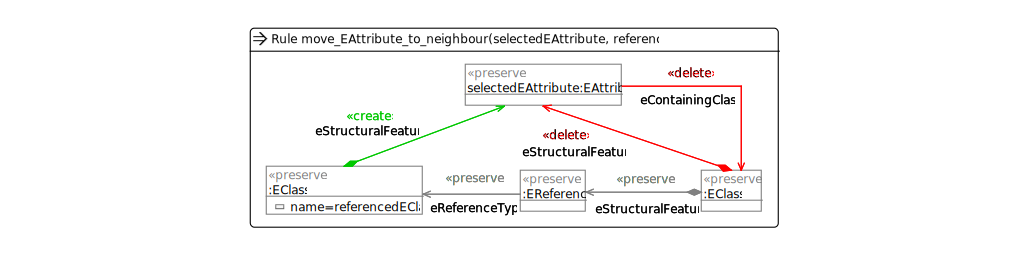
\includegraphics[width=1.0\textwidth]{images/henshin_rule.png}
  \caption{Visueller graphbasierter Henshin Editor}
  \label{fig:henshin_rule}
\end{figure}
\chapter{Differenz Pipeline}
\label{diffPipe}

Die folgenden Abschnitte dokumentieren die Implementierung des in \cite{KeKT2011ASE} beschriebenen
Konzepts des Semantic-Liftings. Die einzelnen Teile des Konzepts werden dabei in Bezug auf
ihre technische Umsetzung nochmal im Detail untersucht. Es wird dabei auch auf aufgetretene Probleme
und ggf. auf deren Lösungsansatz eingegangen.

\begin{figure}[htbp]
  \centering
  \includegraphics[scale=0.2]{images/difference_pipeline.png}
  \caption{Differenz Pipeline \cite{KeKT2011ASE}}
  \label{fig:diff_pipeline}
\end{figure}

Die Architektur des Semantic-Lifting Algorithmus lässt sich als Pipeline beschreiben, wie in
Abbildung \ref{fig:diff_pipeline} dargestellt. Als Eingabe für diese Pipeline dienen immer zwei
Versionen eines Modells. Diese beiden Versionen werden im Folgenden immer als \textbf{Modell A} und
\textbf{Modell B} bezeichnet, wobei Modell A  als die Ausgangsversion des Modells betrachtet wird,
während Modell B eine spätere Version des Modells darstellt, in der im Vergleich zu Modell A
verschiedene Teile hinzugefügt oder entfernt wurden. Als technische Grundlage für die
Implementierung dient das Eclipse Modeling Framework (EMF). Daher können nur Modelle verglichen
werden, die auf dem EMF eigenen Metamodell Ecore basieren. Im Rahmen dieses Proof-Of-Concepts
verwenden wir Ecore direkt als Metamodell für die zu vergleichenden Modelle. Grundsätzlich können
aber auch z.B. auf Ecore basierende UML Klassendiagramme oder Zustandsautomaten als Eingabe dienen,
wie Abbildung \ref{fig:metaebenen} illustriert. In allen Fällen bildet Ecore einen
selbstreferentiellen Abschluss der Abstraktionsebenen als Meta-Metamodell.

\begin{figure}[htbp]
  \centering
  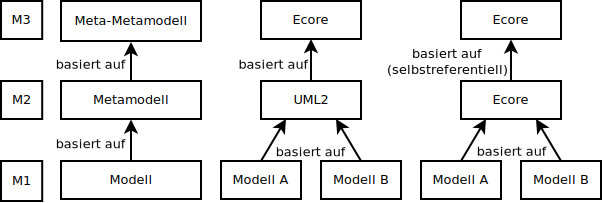
\includegraphics[width=1.0\textwidth]{images/metaebenen.png}
  \caption{Metaebenen}
  \label{fig:metaebenen}
\end{figure}

Die Modelle A und B werden dann in den folgenden Schritten weiter verarbeitet. Der erste Schritt auf
dem Weg zur semantisch gelifteten Differenz ist das Matching (Abschnitt \ref{sec:matching}). In
dieser Phase wird versucht den Elementen aus Modell A die entsprechend gleichen Element aus Modell B
zuzuordnen. Den nächsten Schritt bildet die Differenz-Ableitung (Abschnitt
\ref{sec:diff:derivation}), in der die später zu verarbeitende technische Differenz aus den
Matchings erzeugt wird. Im letzten Schritt erfolgt das Semantic-Lifting (Abschnitt
\ref{sec:lifting}), hier wird aus der technischen Differenz eine semantisch geliftete Differenz
berechnet.

% Matching
\section{Matching}
\label{sec:matching}

Als Matching wird in diesem Zusammenhang der Prozess bezeichnet, in dem die beiden Modelle A und B
miteinander verglichen werden. Dazu werden zustandsbasierte Vergleichsalgorithmen verwendet, welche
eine symmetrische Differenz auf der Basis des aktuellen Zustands der beiden Modelle berechnen.  Ziel
des Matchings ist es herauszufinden welche Elemente in beiden Modellen übereinstimmen. Diese
Übereinstimmungen werden als Korrespondenzen (\textit{engl. Correspondence}) zwischen Modellen A und
B bezeichnet. \cite{KeKT2011ASE} (S.3)

\begin{quote}
\centering
$A \Delta B := \{x \mid (((x \in  A)\wedge(x \not\in B))\vee((x \in B)\wedge(x \not\in A))) \}$
\end{quote}

\begin{figure}[htb]
  \centering
  \includegraphics[scale=0.4]{images/symmetrische_Differenz.png}
  \caption{Symmetrische Differenz}
  \label{fig:sym_diff}
\end{figure}

Die Korrespondenzen geben zunächst die Schnittmenge zwischen den Modellen an. Für die Berechnung der
korrespondierenden Elemente gibt es grundsätzlich verschiedene (zustandsbasierte) Techniken und
Algorithmen:

\begin{itemize}
  \item \textbf{ID-basiert:} In diesem Ansatz wird davon ausgegangen, dass jedes Modell-Element eine
  eindeutige statische ID besitzt. D.h. diese ID wird beim Erzeugen des Elements vergeben und darf
  sich auch im weiteren Entwicklungsverlauf des Modells nicht verändern. Der Hauptvorteil dieses
  Ansatzes besteht darin, dass keine spezielle Konfiguration für unterschiedliche Modelltypen nötig
  ist. Außerdem lassen sich Korrespondenzen sehr effizient berechnen. Dieser Ansatz funktioniert
  allerdings nicht für Modelle, die unabhängig voneinander erzeugt wurden. Außerdem muss die Vergabe
  von IDs durch die verschiedenen Entwicklungsumgebungen gewährleistet sein. \cite{KPRP2009} (S.2)
  
  \item \textbf{Signaturbasiert:} In diesem Ansatz wird eine Signatur zum vergleichen der
  Modell-Elemente verwendet. Im Gegensatz zu einer ID ist die Signatur nicht statisch. Eine Signatur
  wird dynamisch aus den Werten der Eigenschaften eines Elements berechnet. Daher können auf diese
  Weise auch Modelle verglichen werden, die unabhängig voneinander entwickelt wurden. Dieser
  Ansatz ist allerdings mit deutlich mehr Aufwand verbunden, da für jeden Modell-Element-Typ eine
  Berechnungsfunktion für die jeweilige Signatur angelegt werden muss. \cite{KPRP2009} (S.3)
  
  \item \textbf{Ähnlichkeitsbasiert:} In diesem Ansatz werden Modelle als typisierte, attributierte
  Graphen behandelt. Die einzelnen Modell-Elemente werden dabei durch die Summe ihrer Eigenschaften
  identifiziert. Dabei sind nicht alle Eigenschaften gleich wichtig. Hierzu wird in den meisten
  Algorithmen eine Konfiguration benötigt die das relative Gewicht der einzelnen Eigenschaften
  angibt. Herauszufinden welche Gewichtung der Eigenschaften für eine Modellierungssprache ein
  möglichst optimales Ergebnis liefert, ist allerdings häufig ein "`trial-and-error"' Prozess.
  Außerdem können generische Ansätze keine Rücksicht auf die Semantik der Modellierungssprache
  nehmen, welche die Genauigkeit verbessern und die Anzahl der individuellen Vergleiche verringern
  würde. \cite{KPRP2009} (S.3)
  
  \item \textbf{Sprachspezifisch:} Ein sprachspezifischer Matching Algorithmus wurde speziell für
  eine Modellierungssprache implementiert. Da diese Algorithmen die Semantik ihrer
  Modellierungsprache kennen ist hier in der Regel auch kein Semantic-Lifting notwendig. Daher wird
  hier auch nicht näher auf solche Algorithmen eingegangen. Der Nachteil dieses Ansatzes bestehen
  im hohen Entwicklungsaufwand und der auf die Modellierungssprache eingeschränkten Benutzbarkeit.
\end{itemize}
Zur Berechnung der Korrespondenzen für das Semantic-Lifting kann grundsätzlich ein beliebiger
Algorithmus verwendet werden. Die Korrespondenzen müssen nur immer in die interne Darstellung
konvertiert werden. (Siehe \texttt{Correspondeces} Abbildung \ref{fig:diffmodel}.) Ein Vergleich
verschiedener Ansätze ist in \cite{KPRP2009} zu finden. Im folgenden wird nun auf die im Rahmen
dieser Arbeit verwendeten Algorithmen eingegangen.

% Beim Vergleichen von Modellen spielt immer auch die Struktur eine wichtige Rolle. In Ecore werden
% Modelle in Form einer Baumartigen Aggregationsstruktur aufgebaut. Die einzelnen Elemente dieser
% Struktur sind typisiert und ggf. attributiert. Dabei können Elemente dieser Struktur hinzugefügt
% oder entfernt werden. Im Sinne einer Struktur kann man auch von Verschiebung einzelner Elemente
% sprechen, wenn ein Element aus einem Teilbaum einem anderen zugeordnet wird. Die Verschiebung äußert
% sich in einem Modell durch das verändern der Referenzen zwischen Container und Element. Ist das
% Element kein Blatt in der Baumstruktur so können auf diese Weise auch ganze Teilbäume verschoben
% werden. In vielen Fällen kann es wünschenswert sein ein Verschieben als solches zu erkennen und
% nicht als löschen und einfügen von Elementen. In diesem Fall würden dann Korrespondenzen zwischen
% den Verschobenen Elementen bzw. Teilbäumen angelegt, nicht aber zwischen den veränderten Referenzen
% der Container und  der Elemente bzw. Wurzeln der Teilbäume. Korrespondenzen können außerdem
% zwischen nicht gleichen Elementen auftreten. Zum Beispiel kann ein Element auf Grund seiner
% strukturellen Anordnung als Korrespondierend angesehen werden, möglicherweise wurden aber Attribute
% wie der Name des Elements verändert. Auf Grund dieser verschiedenen Eigenschaften muss
% die Menge der Korrespondenzen je nach verwendetem Matching Algorithmus nicht immer Eindeutig sein.

\subsection{SiDiff}
\label{sidiff}

SiDiff ist ein an der Universität-Siegen entwickelter Metamodell unabhängiger Ansatz, um Modelle zu
vergleichen. Der Algorithmus ist hauptsächlich darauf ausgelegt Modell-Elemente nach ihrer
Ähnlichkeit zu vergleichen (ähnlichkeitsbasiert), unterstützt aber auch Ansätze zum ID-basierten
oder signaturbasierten Modellvergleich. Der Hauptvorteil von SiDiff besteht darin, dass dem
Benutzer eine sehr frei konfigurierbare Umgebung geboten wird, die auf jeden Modelltyp angepasst
werden kann. Der Modelltyp muss sich lediglich als graphähnliche Struktur darstellen lassen. Der
generische Algorithmus muss für jeden Modelltyp konfiguriert werden. Eine Konfiguration besteht aus
einer Transformation vom Originaldokument in die interne Repräsentation, einer Definition für die
Gewichtung der Eigenschaften der zu vergleichenden Modell-Elemente für die Berechnung der
Ähnlichkeiten und einer Spezifizierung der auszugebenden Daten. \cite{SiDiff}

% SiDiff is an meta model-independent approach to model comparison. It is primarily based on the
% notion of similarity between model elements, but covers other approaches like id-based or
% signature-based model comparison as well. The main advantage of SiDiff is that it offers a highly
% configurable environment and is therefore easily adaptable to any model type where models can be
% represented in a graph-like structure
% 
% The generic algorithm must be configured for each type of model. A configuration consists of a
% transformations from the original document into an internal structure, the definition of the
% similarity of elements, a specification of the output, and further details.

\subsection{Named-Element-Matcher}
\label{nem}

Der Named-Element-Matcher wurde im Rahmen diese Projekts als Testwerkzeug verwendet, er vergleicht
die beiden Modelle A und B einfach anhand der Namen der einzelnen Elemente. Der Matcher eignet sich
vor allem für selbst konstruierte Testfälle, da das Ergebnis des matchings relativ gut abzusehen
ist. Dieser Algorithmus lässt sich als ein signaturbasierter Algorithmus einordnen. Als Signatur
wird in diesem Fall eben nur der Namen benutzt.


% Differenz-Ableitung
\section{Differenz-Ableitung}
\label{sec:diff:derivation}

Die Differenz-Ableitung ist der zweite Schritt zur Berechnung einer symmetrischen Differenz zwischen
Modell A und B. In diesem Schritt werden die Objekte identifiziert, die nicht in der Schnittmenge
der beiden Modell sind. Die so berechnete Differenz wird im Folgenden als \textbf{technische
Differenz} bezeichnet. Eine technische Differenz teilt sich zunächst in zwei Klassen ein:
\texttt{Correspondence} und \texttt{Change}. Die zuvor im Matching berechneten Korrespondenzen der
Schnittmenge werden durch Objekte der Klasse \texttt{Correspondence} dargestellt. Die Summe aller
\texttt{Correspondence} gibt damit die gemeinsamen Teile von Modell A und Modell B an. Die Teile,
die sich von Modell A zu Modell B unterscheiden, werden durch Objekte der Klasse \texttt{Change}
(Änderung) angegeben. Bei Änderungen an einem Modell unterscheiden wir dabei noch zusätzlich
zwischen den drei Grundelementen eines Modells: Objekte, Referenzen und Attribute. Objekte und
Referenzen können in ein Modell sowohl eingefügt als auch entfernt werden. Ausgehen davon, dass wir
keine mehrwertigen Attribute betrachten, sind hingegen einwertige Attribute durch die Metaklassen
fest vorgegeben und können daher nur einen neuen Wert zugewiesen bekommen. Zu diesem Zweck werden
folgende Klassen definiert:

\begin{itemize}
  \item \texttt{Add-Object}: In Modell B existiert ein Objekt, welches nicht in Modell A existiert.
  Das Objekt wurde also in Modell B hinzugefügt.
  
  \item \texttt{Remove-Object}: In Modell A existiert ein Objekt, welches nicht in Modell B
  existiert. Das Objekt wurde also in Modell B entfernt.
  
  \item \texttt{Add-Reference}: In Modell B existiert eine Referenz, welche nicht in Modell A
  existiert. Die Referenz wurde also in Modell B hinzugefügt.
  
  \item \texttt{Remove-Refernce}: In Modell A existiert eine Referenz, welche nicht in Modell B
  existiert. Die Referenz wurde also in Modell B entfernt.
  
  \item \texttt{Attribute-Value-Change}: Für alle Objekte aus Modell A und Modell B, für die eine
  Korrespondenz existiert, wird überprüft, ob sich der Wert eines Attributs verändert hat und ggf.
  ein Attribute-Value-Change erzeugt. Es werden keine Attribute-Value-Changes für neue
  initialisierte Attribute eines Add-Objects angelegt.
  
  Attribute, deren Metatyp (\texttt{EAttribute}) folgende Eigenschaften haben, können dabei
  vernachlässigt werden, da sich aus diesen Attributen keine direkten Änderungen des Modells
  ableiten lassen:
  
  \begin{itemize}
    \item\texttt{changeable = false} $\to$ Der Wert kann von außen nicht verändert werden. D.h. es
    wird keine \texttt{setXX()} Methode generiert. \cite{SBPM2009} (S. 108)
    
    \item\texttt{transient = true} $\to$  Der Wert wird bei der Serialisierung übergangen und nicht
    mit abgespeichert. \cite{SBPM2009} (S. 108)
    
    \item \texttt{derived = true} $\to$ Gibt an, dass dieser Wert aus anderen Informationen
    abgeleitet wird. Hat aber keinen Einfluss auf die Code Generierung. \cite{SBPM2009} (S. 108)
  \end{itemize}
\end{itemize}
Das in Ecore Implementierte Differenzmodell ist in Abbildung \ref{fig:diffmodel} zu sehen. Es bildet
die Basis für das spätere Semantic-Lifting. Die in dieser Phase berechneten \texttt{Changes} werden
im Folgenden als \textbf{low-level Änderungen} bezeichnet, da die durchgeführten Änderungen am
Modell hier noch auf einer rein technischen Ebene angegeben werden.

\begin{figure}[htb]
  \centering
  \includegraphics[width=1.0\textwidth]{images/difference_model.png}
  \caption{Differenzmodell}
  \label{fig:diffmodel}
\end{figure}

% Semantic-Lifiting
\section{Semantic-Lifting}
\label{sec:lifting}

Als Eingabe für das Semantic-Lifting dient die zuvor berechnete technische Differenz der Modelle A
und B. Die technische Differenz enthält ausschließlich low-level Änderungen, welche angeben, was
sich zwischen Modell A und Modell B verändert hat. Da low-level Änderungen auf Basis des Metamodells
angegeben werden, sind diese aber für normale Benutzer oft sehr unverständlich. Auch um einen
schnellen Überblick über die Veränderungen eines Modells zu bekommen, eignet sich diese Form der
Repräsentation nicht besonders gut, da die low-level Änderungen unstrukturiert in der Differenz
liegen. Aus Benutzersicht wäre es wünschenswert die low-level Änderungen so zu strukturieren, dass
sie den Bearbeitungsprozess eines Editors wiedergeben. Genau dieses Ziel verfolgt das
Semantic-Lifting, die technischen Änderungen wieder als Editieroperation auf einer Benutzer
verständlichen Ebene darzustellen. 

Um eine Editieroperation darzustellen, werden die low-level Änderungen neu strukturiert. Jede
angewendete Editieroperation lässt sich auf ein bestimmtes Muster in der Differenz zurückführen.
Dieses Muster besteht sowohl aus low-level Änderungen als auch aus einem bestimmten Kontext. Der
Kontext einer Editieroperation gibt zum einen an, auf welche Elemente die Editieroperation
angewendet werden soll, zum andern können bestimmte Umstände vorgegeben sein, damit der Vorgang
ausgeführt werden darf. Welche Änderungen in welchem Kontext von einer Editieroperation ausgeführt werden, wird
durch die s.g. \textbf{Editierregel} vorgegeben. Aus dieser Editierregel kann dann das Muster
abgeleitet werden, das die Editieroperation in einer Differenz wieder erkennt. Dieses Muster wird
als \textbf{Erkennungsregel} bezeichnet. Das Muster einer Erkennungsregel überprüft die Differenz sowohl
auf auftretende low-level Änderungen als auch auf den Kontext der entsprechenden Editieroperation.
Nachdem also eine bestimmte Editieroperation in der Differenz erkannt wurde, können die
entsprechenden low-level Änderungen der Editeroperation wieder zugeordnet werden. Um diese
semantische Zuordnung von Editieropration zu low-level Änderungen in der Differenz zu speichern,
wird eine neu Klasse in unser Differenzmodell eingeführt. Wie in Abbildung \ref{fig:scs} zu sehen
ist, gruppiert ein s.g. \textbf{Semantic-Change-Set} mehrere zu einer Editieroperation gehörenden
low-level Änderungen (\texttt{Change}). Der Name des Semantic-Change-Sets entspricht der
assoziierten Editieroperation. Dabei ist darauf zu achten, dass am Ende des Semantic-Lifitngs jede
low-level Änderung nur in einem Semantic-Change-Set enthalten ist. Im Semantic-Lifting Konzept  wird
dies wie folgt formuliert:
\begin{quote}
"`The objective of semantically lifting a model difference is thus to partition the set of low-level
changes into disjoint subsets, each subset containing the changes belonging to exactly one edit
operation. These subsets must be disjoint since each low-level change results from the application
of exactly one edit operation. We call these subsets \textbf{semantic change sets}."'
\cite{KeKT2011ASE} (S.5)
\end{quote}

\begin{figure}[htb]
  \centering
  \includegraphics[scale=0.5]{images/semantic_change_set.png}
  \caption{Semantic-Change-Set}
  \label{fig:scs}
\end{figure}
\chapter{Erstellen der Editierregeln}
\label{editierregeln}

Um Modelle bearbeiten zu können, benötigen wir darauf ausgelegte Werkzeuge. In der Regel werden dazu
grafische Editoren oder Transformationstechniken benutzt. Welche Technik zur Bearbeitung eines
Modells verwendet wurde und welche Semantik hinter den einzelnen Veränderungen im Modell steckt, ist
zum Zeitpunkt der Differenzberechnung nicht mehr direkt nachzuvollziehen. Das Problem ist, dass dem
generischen Differenzberechner keine Informationen über die Semantik der möglichen
Editieroperationen vorliegt. Um die Semantik wiederherzustellen, müssen wir allerdings wissen,
welche Editieroperationen für einen bestimmten Modelltyp existieren und wie diese aussehen. Hierzu
werden s.g. Editierregeln verwendet. Die Editierregeln sind die Grundlage für das spätere Semantic-Lifting.
Eine Editierregel beschreibt eine Editieroperation, die vom Entwickler auf einem Modell eines
bestimmten Typs ausgeführt werden kann. Dabei hat jeder Modelltyp auf Basis seines Metamodells und der
Semantik andere Editieroperationen. Daher müssen auch die Editierregeln für jeden Modelltyp einzeln
angegeben werden.

\section{Identifikation von Editierregeln}

Zunächst stellt sich an dieser Stelle die Frage, welche Editierregeln benötigt werden, um das
vollständige Bearbeiten eines Modells zu ermöglichen. Grundsätzlich können hier natürlich
verschiedene Ansätze gewählt werden. Eine Möglichkeit wäre es, falls vorhanden, den Editor für den
bestimmten Modelltyp zu analysieren und festzustellen, welche Editieroperationen zur Verfügung
gestellt werden. Eine weitere Möglichkeit besteht darin, das eigentliche Metamodell und die damit
verbundenen Constraints zur Erstellung der Editierregeln zu verwenden.

Da das Semantic-Lifting ein generischer Ansatz ist, kann zu diesem Zeitpunkt noch keine Aussage über
die später in der Praxis verwendeten Metamodelle getroffen werden. Die eigentliche Entscheidung,
welche Editierregeln benötigt werden und wie diese aussehen, bleibt damit zum Teil auch dem
Entwickler überlassen, der die Semantic-Lifting-Engine für ein bestimmtes Metamodell
konfiguriert. Dabei sollte bedacht werden, dass eben nicht immer eindeutig klar ist, auf welche Art
das Modell bearbeitet wurde. Unterschiedliche Editoren können für ein und dasselbe Metamodell
unterschiedliche Editieroperationen haben.

Die Editierregeln müssen also alle Editieroperationen nachbilden, die grundlegend möglich wären.
Trivial aber entscheidend an dieser Stelle ist, dass später nur solche Editieroperationen geliftet
werden, für die auch eine Editierregel oder eine entsprechende Zerlegung von mehreren Editierregeln
existiert. Aufgrund dieser Überlegungen erschien eine Analyse des Metamodells zur Ableitung der
Editierregeln am sinnvollsten. An Hand des Metamodells lässt sich am besten schematisch und formal
nachvollziehen, welche Editierregeln benötigt werden. Allgemein formuliert werden zunächst die
Editierregeln benötigt, mit denen für ein Modell neue Elemente erzeugt, bestehende Elemente entfernt
oder ggf. abgeändert werden können. Ziel ist es eine Basismenge an Editierregeln zu erzeugen, die
sich an folgende Definition anlehnt. Statt \textit{"`atomic pattern"'} wird hier im Folgenden der
Begriff der \textbf{Atomic-Editierregel} verwendet:

\begin{quote}
"`Atomic patterns constitute basic elements for composing modeling patterns. They are governed by
two characteristics: On the one hand, they maintain model consistency, of course. On the other hand,
they cannot be split into smaller modeling patterns keeping model consistency. Therefore, they form
the smallest units of consistent model changes.

By using atomic patterns only, it is possible to create all eligible instances of a specific
modeling language. E.g., for each model element defined by the modeling language, at least one
particular atomic modeling pattern exists performing the minimum of required modeling steps to
create this model element. Otherwise this model element is no eligible element of the modeling
language, e.g. due to prohibition by constraints."' \cite{W2010} (S.11)
\end{quote}

\section{Editierregeln für Ecore}

Betrachtet man das Ecore Metamodell (Abbildung \ref{fig:ecore_metamodel}), so lassen sich 69
Atomic-Editier"-regel identifizieren. Abstrakte Klassen (nicht deren Attribute und Referenzen),
abgeleitete Referenzen und nicht veränderbare Attribute müssen nicht betrachtet werden. Die Regeln
sollen wie in der Definition beschrieben, die Konsistenz des Modells aufrecht erhalten. Man muss
bedenken, dass die Ecore Editoren auch Editieroperationen zulassen, die das Modell inkonsistent
werden lassen. Zum Beispiel können Klassen ohne Namen oder Attribute ohne Typ angelegt werden. Die
Atomic-Editierregeln lassen sich wie unten aufgelistet in mehrere Kategorien einteilen. Die
Aufteilung in diese Kategorien dürfte sich aber in der Regel auch auf jeden anderen Modelltyp
übertragen lassen.

\begin{itemize}
  \item \textbf{11 $\times$ Add <Class>:} Hinzufügen eines Modell-Elements.
  \item \textbf{11 $\times$ Remove <Class>:} Entfernen eines Modell-Elements.
  \item \textbf{11 $\times$ Move <Class>:} Verschieben eines bestehenden Modell-Elements.
  \item \textbf{5 $\times$ Add Reference <Class> <Reference>:} Hinzufügen einer optionalen Referenz zu
  einem bestehenden Modell-Element.
  \item \textbf{5 $\times$ Remove Reference <Class> <Reference>:} Entfernen einer optionalen Referenz zu
  einem bestehenden Modell-Element.
  \item \textbf{3 $\times$ Change Reference <Class>:} Verändern einer benötigten Referenz eines
  bestehenden Modell-Elements.
  \item \textbf{23 $\times$ Attribute Value Change <Class> <Attribute>:} Ändern eines Attributs eines
  bestehenden Modell-Elements.
\end{itemize}
Regeln, die nicht in die Kategorie der Atomic-Editierregel fallen, werden im Folgenden als
\textbf{Advanced-Editierregel} bezeichnet. Eine Advanced-Editierregel kann im Prinzip als eine
Zusammensetzung bzw. Spezialisierung von Atomic-Editierregeln betrachtet werden.

% Der Editieranteil einer Advanced-Editierregel muss sich in mehrere Atomic-Editierregel zerlegen
% lassen. D.h. eine Advanced-Editierregel kann ggf. noch zusätzliche Einschränkungen dahingehend
% enthalten, dass ein bestimmter Zustand des Modells gegeben sein muss damit die Regel angewendet
% werden kann.

% 18 Advanced-Edit-Rules:
% 
% \begin{itemize}
% \item Create/Remove referenced EClass
% \item Create/Remove sub EClass
% \item Create/Remove super EClass
% \item Move EAttribute to neigbour
% \item Pull up EAttribute
% \item Push down EAttribute
% \item Rename EAttribute/EClass/EDataType/EEnum/EEnumLiteral/EOperation/
% EPackage/EParameter/EReference
% \end{itemize}

\section{EMF-Refactor}

Um die Editierregeln zu formulieren werden Henshin Transformationssysteme (TS) verwendet. Diese
Transformationssysteme müssen bestimmten Konventionen entsprechen, damit sie später für das
Semantic-Lifting weiterverarbeitet werden können. Die Konventionen entsprechen denen von
EMF-Refactor Regeln. EMF-Refactor ist ein Werkzeug um benutzerdefinierte Refactorings für Ecore
basierte Modelle anzulegen. Die einmal angelegten Refactorings können dann über den baumbasierten
EMF-Editor auf das Modell angewendet werden.  Der Unterschied zwischen einem Refactoring und einer
Editieroperation besteht darin, dass ein Refactoring nur die Struktur des Modells verändert, nicht
aber das Verhalten wie bei einer Editieroperation. Der Aufbau von Editierregeln für
Editieroperationen unterscheidet sich aber nicht von dem für Refactorings, daher lässt sich das
Konzept problemlos übernehmen. EMF-Refactor definiert drei Henshin Transformationssysteme, aus denen
ein Refactoring besteht.

\begin{itemize}
  \item \textbf{Initial-Check-TS} (\textit{Precondition})\textbf{:} Hier werden grundlegende Tests
  durchgeführt, ob das Refactoring angewendet werden darf. Dazu wird für jede Situation, in der das
  Refactoring nicht angewendet werden darf, eine Regel formuliert. In diesen Regeln wird genau die
  Situation dargestellt, die nicht auftreten darf. Das Refactoring darf nur dann ausgeführt werden,
  wenn keine Initial-Check-Regel zutrifft, bzw. anwendbar ist. Dazu wird eine Independent-Unit
  verwendet, die alle Regeln enthält. Eine Independent-Unit ist dann anwendbar, wenn genau eine
  Regel der Unit anwendbar ist. D.h. die Independent-Unit darf zum ausführen des Refactorings nicht
  anwendbar sein. Theoretisch können auch mehrere Units verschachtelt werden. Um dem EMF-Refactor
  kenntlich zumachen, welche Unit beim Initial-Check ausgeführt werden soll, muss diese Unit mit dem
  Namen \textit{mainUnit} gekennzeichnet werden.
  
  \item \textbf{Final-Check-TS}  (\textit{Precondition})\textbf{:} Der Final-Check unterscheidet
  sich strukturell nicht vom Initial-Check. Auch hier muss es eine Unit mit Namen \textit{mainUnit} 
  geben, die nicht anwendbar sein darf, damit das Refactoring durchgeführt werden kann. Im
 Unterschied zum Initial-Check wird der Final-Check durchgeführt, nachdem die für das Refactoring
 benötigten Daten vom Benutzer abgefragt wurden. Hier wird überprüft, ob die eingegebenen Daten für
 das Refactoring verwendet werden können. Zum Beispiel könnte beim Erstellen einer Klasse überprüft
 werden, ob eine Klasse mit dem gleichen Namen schon existiert.
 
  \item \textbf{Execute-TS:} In der Execute Phase wird das eigentliche Refactoring ausgeführt. Die
  in diesem Transformationssystem enthaltenen Regeln geben an, welche Änderungen an dem Modell
  durchgeführt werden sollen. Auch hier muss wieder eine \textit{mainUnit} spezifiziert werden.
\end{itemize}
Für das Semantic-Lifting ist hauptsächlich das Execute-TS von Bedeutung. Das Refactoring für eine
bestimmte Modellierungssprache wird hier auf Basis des Metamodells angegeben. Daher lassen sich aus
den Regeln die eigentlichen low-level Änderungen ablesen, die durch das Semantic-Lifting wieder
erkannt werden sollen. Im Fall des Initial- und Final-Check gehen wir zunächst einmal davon aus,
dass, wenn ein angewandtes Refactoring erkannt wurde, auch die Vorbedingungen
(\textit{engl. precondition}) für dieses Refactoring erfüllt waren.

Damit die Henshin Transformationssysteme durch die Semantic-Lifting-Engine verarbeitet werden
können, müssen diese den EMF-Refactor Konventionen entsprechen. Genauere Angaben und Beispiele sind
auf \cite{ERe} zu finden.

\chapter{Generieren der Erkennungsregeln}
\label{generierung}

Ziel des Semantic-Liftings ist es, die low-level Änderungen der technischen Differenz wieder einer
bestimmten Editieroperation zuzuordnen. Die Änderungen einer Editieroperation werden durch die
Editierregeln vorgegeben. Das Auslesen der Editieroperation aus der Differenz wird durch die s.g.
Erkennungsregeln erledigt. Eine Erkennungsregel ordnet den low-level Änderungen wieder eine
Editieroperation zu und gruppieren diese in s.g. Semantic-Change-Sets. Die Erkennungsregeln sind,
genau so wie die Editierregel, Henshin Transformationssysteme. Alle Informationen, die für die
Erkennung der Editieroperation benötigt werden, sind in der Editierregel vorhanden und deren
Semantik ist wohldefiniert. Für jeden Teil einer Editierregel lässt sich eindeutig nachvollziehen,
welche Änderungen dadurch in der Differenz auftreten werden. Daher können die Erkennungsregeln
vollständig automatisch aus den Editierregeln generiert werden. Diese Aufgabe übernimmt der
\textbf{Erkennungsregel Generator}.
\begin{quote}
"`Change set recognition rules are getting complex very quickly. However, they are very schematic
and can be automatically generated from their corresponding edit rule."' \cite{KeKT2011ASE} (S.6)
\end{quote}

\section{Implizite Kanten}
\label{implicit_edge}

Bevor die eigentliche Generierung der Erkennungsregel beginnen kann, muss die Editierregel ggf. noch
um bestimmte Kanten erweitert werden. In Ecore kann einer Referenz eine entgegen gerichtete Referenz
(\texttt{eOpposite}) zugeordnet werden. In den meisten Fällen reicht es in Henshin aus, wenn eine
Referenz nur in eine Richtung angegeben wird. Die entgegen gerichtete Referenz wird dann, z.B. beim
erzeugen einer Referenz, automatisch mit eingefügt.

\begin{figure}[htbp]
  \centering
  \includegraphics[scale=0.8]{images/add_eclass.png}
  \caption{Ecore Klasse einfügen}
  \label{fig:add_eclass}
\end{figure}

Im Beispiel in Abbildung \ref{fig:add_eclass} wird eine neue Klasse in ein Paket eingefügt. Beim
einfügen neuer Objekte in ein Ecore Modell wird typischerweise eine Referenz sowohl zwischen
Container und Objekt als auch zwischen Objekt und Container erzeugt. Angegeben wurde in diesem Fall
aber nur die Referenz \texttt{eClassifiers} vom Container zum Objekt. Diese Referenz besitzt aber
eine entgegen gerichtete Referenz \texttt{ePackage} vom Objekt zum Container. Eben genau diese
low-level Änderungen werden nach Anwendung dieser Regel in der technischen Differenz auftreten: 2
$\times$ Add-References und 1 $\times$ Add-Object.

Das Problem solcher \textbf{impliziten Kanten} kann wie schon angedeutet in Ecore häufiger
auftreten. Damit alle Änderungen durch die Erkennungsregel wieder vollständig zugeordnet werden
können, müssen zunächst alle impliziten Kanten in den Transformationsgraphen eingefügt werden. Dazu
werden folgende Schritte für alle Kanten im Graphen ausgeführt:

\begin{enumerate}
  \item Besitzt der Typ (\texttt{EReference}) der aktuellen Kante $X$ eine entgegen gerichtete
  Referenz (\texttt{eOpposite})?
  \item Ist dies der Fall, dann überprüfe, ob eine Kante $Y$ existiert, die in entgegengesetzter
  Richtung zur Kante $X$ verläuft und vom entsprechenden \texttt{eOpposite} Typ ist.
   \item Wurde Kante $Y$ nicht gefunden, dann füge sie dem Graphen hinzu.
\end{enumerate}
Nachdem alle impliziten Kanten eingefügt wurden, kann mit der eigentlichen Erkennungsregel
Generierung begonnen werden.

\section{Parameter}
\label{parameter}

Die Parameter der Editierregel werden zu Beginn vollständig in die Erkennungsregel übernommen. Sie
lassen sich dabei in zwei Kategorien einteilen:

\begin{itemize}
  \item \textbf{Regel-Parameter:} Parameter wird innerhalb der Regel durch ein Attribut eines Knoten
  initialisiert.
  \item \textbf{Unit-Parameter:} Parameter wird von außen an die Regel übergeben. D.h es wird ein
  benutzerdefinierter Wert vor Aufruf der Regel gesetzt. Dies ist im Fall einer EMF-Refactor
  Regel immer ein Parameter, der auf einen Parameter der  \textit{mainUnit} gemappt wurde.
\end{itemize}
Diese Unterscheidung spielt innerhalb der Erkennungsregel beim vergleichen der Attributwerte eine
Rolle. Der ursprüngliche Wert eines Unit-Parameters, der der Editierregel übergeben wurde, ist in
der Erkennungsregel nicht mehr bekannt. Problematisch wird dies dann, wenn der Wert des Unit-Parameters
durch einen bestimmten Ausdruck mit anderen Parametern oder Werten verrechnet wurde (z.B.
\texttt{+,-,*,/}). Um den Wert des Unit-Parameter wieder zu extrahieren, würde man die entsprechende
Umkehrfunktion zu diesem Ausdruck benötigen, bzw. man müsste diesen automatisch berechnen. In
Henshin ist es allerdings nur möglich, Attributwerte auf einfache Gleichheit zu überprüfen. Reguläre
Ausdrücke oder ähnliches, um z.B. eine String Konkatenation zu überprüfen, sind nicht möglich.
Ausdrücke in denen Unit-Parameter verrechnet werden, werden daher bei der Generierung bisher
übergangen.

\section{Generierungsmuster}
\label{patterns}

Um aus einer Editierregel eine Erkennungsregel zu generieren, werden jeweils die einzelnen Elemente
eines Henshin Transformationssystems betrachtet. Ein Transformationssystem besteht aus einem linken
(\textit{Left-Hand Site} (LHS)) und einem rechten Graph (\textit{Right-Hand Site} (RHS)). Dieser
besitzt wiederum: Knoten (\textit{engl. Node}), Kanten (\textit{engl. Edge}) und Attribute
(\textit{engl. Attribute}). Alle diese Elemente können sowohl nur auf der linken
(\texttt{<<delete>>}) als auch nur auf der rechten Seite (\texttt{<<create>>}) oder auch auf beiden
Seiten (\texttt{<<preserve>>})  der Regel vorkommen. Diese Stereotype werden im Folgenden verwendet,
um die Zuordnung eines Henshin Elements zu einer bestimmten Seite der Regel auszudrücken. In der
grafischen Henshin Notation dargestellt ergeben sich damit die folgenden Muster, um Elemente einer
Editierregel in eine Erkennungsregel zu transformieren. Die Editierregel Muster sind jeweils links
und die Erkennungsregel-Muster jeweils rechts dargestellt. Das fiktive Metamodell in Abbildung
\ref{fiktiv_metamodel} dient als Beispiel für die abgebildeten Muster.

\begin{figure}[htbp]
  \centering
  \includegraphics[scale=0.65]{images/fiktiv_metamodel.png}
  \caption{Fiktives Metamodell}
  \label{fiktiv_metamodel}
\end{figure}

\begin{itemize}
  \item \textbf{Remove-Object-Pattern:} Für jeden Knoten, der nur auf der linken Seite der Regel
  vorkommt, wird das Muster in Abbildung \ref{pattern_remove_object} erzeugt. Ein Remove-Object
  zeigt auf ein Objekt aus Modell A vom entsprechenden Typ.
  
  \begin{figure}[htbp]
    \centering
    \includegraphics[scale=0.8]{images/pattern_remove_object.png}
    \caption{Remove-Object-Pattern}
    \label{pattern_remove_object}
  \end{figure}
  
  \item  \textbf{Add-Object-Pattern:} Analog zum Remove-Object-Pattern wird das Add-Object-Pattern
  für jeden Knoten angelegt, der nur auf der rechten Seite der Regel vorkommt. Das referenzierte
  Objekt ist in diesem Fall aus Modell B.
  
  \begin{figure}[htbp]
    \centering
    \includegraphics[scale=0.8]{images/pattern_add_object.png}
    \caption{Add-Object-Pattern}
  \end{figure}
  
  \item \textbf{Correspondence-Pattern:} Innerhalb der Differenz werden durch dieses Muster genau
  die Teile ausgewählt, die sich von Modell A zu Modell B nicht verändert haben. Dazu wird durch
  einen \textbf{Correspondence-Knoten} ein Objekt aus Modell A mit dem entsprechenden Objekt aus
  Modell B verbunden. Siehe Abbildung \ref{fig:pattern_correspondence}. Dieses Muster tritt immer
  dann auf,  wenn ein Knoten auf beiden Seiten der Editierregel vorkommt (\texttt{<<preserve>>}).
  Knoten, die Objekte aus Modell A bzw. Modell B repräsentieren, werden im Folgenden als
  \textbf{Modell A Knoten} bzw. \textbf{Modell B Knoten} bezeichnet.
  
  \item \textbf{Preserved-Reference-Pattern:} Genau so wie \texttt{<<preserve>>} Knoten in der
  Editierregel durch \texttt{<<preserve>>} Kanten verbunden werden, werden auch die entsprechend
  Modell A und B Knoten der Correspondence-Patterns verbunden.
  
  \begin{figure}[htbp]
    \centering
    \includegraphics[scale=0.8]{images/pattern_correspondence.png}
    \caption{Correspondence- \& Preserved-Reference-Pattern}
    \label{fig:pattern_correspondence}
  \end{figure}
 
  \item \textbf{Remove-Reference-Pattern:} Als nächstes werden nun die Kanten betrachtet, die nur
  auf der linken Seite (\texttt{<<delete>>}) der Regel  vorkommen. Eine Remove-Reference verbindet durch
  Quelle (\texttt{src}) und Ziel (\texttt{tgt})  immer zwei Modell A Knoten. D.h., werden die Muster
  beim generieren in der hier beschriebenen Reihenfolge abgearbeitet, so wurden die Knoten $A1$ und
  $A2$ bereits durch Correspondence-Patterns oder durch Remove-Object-Patterns erzeugt, da sich die
  Muster an dieser Stelle überschneiden. Welche Muster sich überschneiden, hängt eben davon ab, ob
  die Knoten der Editierregel \texttt{<<preserve>>} oder \texttt{<<delete>>} Knoten sind. Der Fall eines
  \texttt{<<create>>} Knoten in Verbindung mit einer \texttt{<<delete>>} Kante ist nicht möglich und
  muss daher nicht betrachtet werden.
  
  Neben Quelle und Ziel der Editierregel Kante muss in der Erkennungsregel noch der Typ betrachtet
  werden. Dazu wird das Meta-Metamodell, also Ecore, verwendet und der Typ der Remove-Reference auf
  eine \texttt{EReference} mit dem entsprechenden Namen geprüft. Grundsätzlich könnte es vorkommen, dass
  eine Referenz mit dem gleichen Namen im Metamodell mehrfach existiert. Der Kontext für die
  Referenz wird aber eindeutig durch die Quelle (\texttt{src}) der Remove-Reference vorgegeben. Ein
  solcher Knoten zur Überprüfung des Typs wird im Folgenden als \textbf{Typknoten} bezeichnet.
  
  \begin{figure}[htbp]
    \centering
    \includegraphics[scale=0.8]{images/pattern_remove_reference.png}
    \caption{Remove-Reference-Pattern}
  \end{figure}
  
  \item \textbf{Add-Reference-Pattern:}  Für das Add-Reference-Pattern werden analog zum
  Remove-Reference-Pattern die Kanten betrachtet, die nur auf der rechten Seite
  (\texttt{<<create>>}) der Editierregel vorkommen.
  
  Innerhalb der Editierregel können \texttt{<<create>>} Kanten nur zwischen \texttt{<<create>>} oder
  \texttt{<<preserve>>} Knoten auftreten.  Damit zeigen die \texttt{src} und \texttt{tgt} Kanten des
  Add-Reference Knoten immer auf Modell B Koten. Entsprechend dem Remove-Reference-Pattern wurden
  die Modell B Knoten $B1$ und $B2$ bereits von Correspondence-Patterns oder von
  Add-Object-Patterns erzeugt.
  
  \begin{figure}[htbp]
    \centering
    \includegraphics[scale=0.8]{images/pattern_add_reference.png}
    \caption{Add-Reference-Pattern}
  \end{figure}

  \item \textbf{Attribute-Value-Change-Pattern:} Dieses Muster wird nur auf Attribute angewendet,
  die Teil eines \texttt{<<preserve>>} Knoten sind. Für Attribute, die beim neu Anlegen von Objekten
  gesetzt werden, werden bei der Differenz-Ableitung keine Attribute-Value-Changes erzeugt.
  D.h. \texttt{<<create>>} Knoten und deren Attribute müssen nicht beachtet werden.
  
  Daher verbindet das Attribute-Value-Change-Pattern immer ein Objekt aus Modell A mit dem
  entsprechenden Objekt aus Modell B. Das bedeutet für diesen Fall, dass die Knoten $A1$ und $B1$
  bereits durch ein Correspondence-Pattern angelegt wurden. Der Typ des Attributs wird, ähnlich wie
  der Referenztyp beim Remove-Reference-Pattern, durch einen \texttt{EAttribute} Typknoten mit
  Hilfe des Namens überprüft.
  
  \begin{figure}[htbp]
    \centering
    \includegraphics[scale=0.8]{images/pattern_attribute_value_change.png}
    \caption{Attribute-Value-Change-Pattern}
  \end{figure}
  
  Zusätzlich wird in der Erkennungsregel noch der Wert, der in der Editierregel angegebenen
  Attribute überprüft. Handelt es sich um feste primitive Werte, also z.B. Zeichenketten oder
  Zahlen, kann damit im ersten Fall überprüft werden, ob sich der Wert im Modell A Objekt von
  \textit{valueX} zu \textit{valueY} im Modell B Objekt verändert hat. Im zweiten Fall tritt das
  Attribut nur auf der rechten Seite der Regel (\texttt{<<create>>}) auf, hier würde das Attribut
  nur für den Modell A Knoten (Knoten $A1$) angelegt und überprüft.
  
  Handelt es sich hingegen bei den Henshin Attributwerten um Parameter, so würde dadurch bei
  mehrfachem Auftreten eines Parameters in verschiedenen Attributen überprüft, ob die jeweiligen
  Werte gleich sind. Neben einzelnen primitiven Werten und Parametern können für Henshin Attribute
  auch komplexere \textit{JavaScript} Ausdrücke mit Parametern, Werten und Operatoren angelegt
  werden. Für solche Ausdrücke gelten die zuvor im Abschnitt \ref{parameter} beschriebenen
  Einschränkungen für Unit-Parameter. Dies gilt auch für alle folgenden Attribute-Value-Patterns.
  
  \item \textbf{Add-Attribute-Value-Pattern:} Wie bereits erwähnt werden für neu angelegte Objekte
  keine Attribute-Value-Changes berechnet. Das Attribut wird aber wieder für das entsprechende
  Modell B Objekt geprüft.
   
  \begin{figure}[htbp]
    \centering
    \includegraphics[scale=0.8]{images/pattern_add_attribute_value.png}
    \caption{Add-Attribute-Value-Pattern}
  \end{figure}
   
  \item \textbf{Remove-Attribute-Value-Pattern:} Dieses Muster wird analog zum
  Add-Attri"-bute-Value-Pattern für aus Modell A entfernte Objekte angelegt.
  
  \begin{figure}[htbp]
    \centering
    \includegraphics[scale=0.8]{images/pattern_remove_attribute_value.png}
    \caption{Remove-Attribute-Value-Pattern}
  \end{figure}
  
  \item \textbf{Preserved-Attribute-Value-Pattern:} Beim Preserved-Attribute-Value-Pattern wird
  überprüft, dass sich ein Wert von Modell A zu Modell B nicht ändert. Dazu wird das
  gleiche Attribut sowohl für den Modell A  Knoten als auch für Modell B Knoten angelegt. Ein
  \texttt{<<delete>>} Attribut in einem \texttt{<<preserve>>} Knoten verhält sich dabei in Henshin
  ganuso wie ein \texttt{<<preserve>>} Attribut.
  
%   \begin{centering}
%     \includegraphics[scale=0.78]{images/pattern_preserve_attribute_value.png}\\
%     \stepcounter{figure}
%     Abbildung \thefigure: Preserved-Attribute-Value-Pattern\\
%   \end{centering}
  
  \begin{figure}[htbp]
    \centering
    \includegraphics[scale=0.8]{images/pattern_preserve_attribute_value.png}
    \caption{Preserved-Attribute-Value-Pattern}
    \label{avc-preserve}
  \end{figure}
  
  \item \textbf{Semantic-Change-Set-Pattern:} Abschließend muss noch der
  \textbf{Differenz-Kno"-ten} und der \textbf{Semantic-Change-Set-Knoten} angelegt und mit allen \textbf{Änderungsknoten}
  (Add/Remove-Object-Knoten, Add/Remove-Reference-Knoten und Attribute-Value-Change-Knoten)
  verbunden werden. Für das Semantic-Change-Set werden noch die drei folgenden Attribute angelegt und
  initialisiert: \texttt{name}, \texttt{priority} und \texttt{refinementLevel}. Der Name des
  Semantic-Change-Sets entspricht der ursprünglichen Editierregel. Auf die Attribute
  \texttt{priority} und \texttt{refinementLevel} wird später im Rahmen des Abschnitts
  \ref{post_processing} Post-Processing noch genauer eingegangen.

  \begin{figure}[h!]
    \centering
    \includegraphics[scale=0.8]{images/pattern_semantic_change_set.png}
    \caption{Semantic-Change-Set-Pattern}
  \end{figure}
  
\end{itemize}

\subsection{Traces}
\label{traces}

Grundsätzlich ist die Reihenfolge, in der die Muster abgearbeitet werden, voneinander unabhängig.
Da die einzelnen Muster aber über die Modell A und B Knoten zusammenhängen, bietet es sich an zunächst
die Remove/Add-Object- und Correspondence-Patterns zu erzeugen. Damit eine korrekte Zuordnung der
sich überschneidenden Knoten zwischen den einzelnen Muster möglich ist, muss abgespeichert werden,
welcher Modell A und B Knoten der Erkennungsregel welchem Knoten der Editierregel entspricht. Diese
Zugehörigkeit von Knoten wird im Folgenden als \textbf{Trace} bezeichnet.

\subsection{Typknoten}
\label{typknoten}

Eine weitere Überschneidung kann bei den Typknoten der Remove-Reference-Patterns und
Add-Reference-Patterns oder beim Attribute-Value-Change-Pattern auftreten. Da der Henshin Graph
injektiv auf den Arbeitsgraphen abgebildet wird, darf auch jeder Typknoten, der ein bestimmtes
Element des Metamodells darstellt, nur einmal erzeugt werden. 

\subsection{Generierungsbeispiel}
\label{gen_example}

Die Muster müssen auf alle Elemente in einer Editierregel angewandt werden, um die zugehörige
Erkennungsregel zu generieren. In Abbildung \ref{fig:add_eclass_recognition} ist die generierte
Erkennungsregel (unten) zu der Editierregel \textit{add empty EClass} (oben) abgebildet. In diesem
Fall lassen sich vier Generierungsmuster identifizieren:

\begin{itemize}
  \item 1 $\times$ Correspondence-Pattern markiert mit (1).
  \item 2 $\times$ Add-Reference-Pattern. Die Referenz \texttt{eClassifiers} wurde mit (2) markiert.
  Die Referenz \texttt{ePackage} ist eine implizite Kante und daher nicht in der Editierregel zu sehen.
  \item 1 $\times$ Add-Object-Pattern markiert mit (3).
\end{itemize}

\begin{figure}[htbp]
  \centering
  \includegraphics[width=1.0\textwidth]{images/add_eclass_recognition.png}
  \caption{Add \texttt{EClass} Erkennungsregel}
  \label{fig:add_eclass_recognition}
\end{figure}

% Dazu werden bei der Generierung alle bereits erzeugten Typknoten in einer Liste abgespeichert,
% sodass nur bei Bedarf neue Typknoten angelegt werden.

\section{Amalgamation Units}

Eine Amalgamation Unit besteht immer aus genau einer Kernregel und beliebig vielen Multiregeln.
Um eine Amalgamation Unit von einer Editierregel in eine Erkennungsregel zu transformieren, muss
die Kernregel und jede einzelne Multiregel nach dem zuvor beschriebenen Verfahren in eine
Erkennungsregel transformiert werden. \texttt{editR2RecognR()} im Pseudocode in Abbildung
\ref{fig:amalgamtion_code}

\begin{figure}[htbp]
  \centering
  \includegraphics[scale=0.18]{images/amalgamation_code.png}
  \caption{Amalgamation Unit Generierung \cite{KeKT2011ASE} (S.7)}
  \label{fig:amalgamtion_code}
\end{figure}

Der nächste Schritt ist dann das Erzeugen der Mappings zwischen Kernregel und Multiregeln.
\texttt{embedKernel()} im Pseudocode in Abbildung \ref{fig:amalgamtion_code}. D.h.
für jeden Knoten einer Multi-Erkennungsregel wird ein Mapping auf einen Knoten der
Kern-Erkennungsregel angelegt. Das Mapping zwischen einer Multi-Erkennungsregel und einer
Kern-Erken"-nungsregel lässt sich nur dann vollständig angeben, wenn die entsprechende
Multi-Editierregel die Kern-Editierregel als Teilgraph enthält. Dies gilt sowohl für Knoten als
auch für Kanten.

Das Problem beim Anlegen der Mappings besteht darin, dass aus einem Knoten einer Editierregel immer
mehrere Knoten in der Erkennungsregel resultieren. Für alle Kanten besteht das gleiche Problem.
Außerdem existieren für Kanten keine expliziten Mappings. Es wäre also rein technisch nicht
unmöglich in einer Multiregel eine Kante anzulegen, die nicht in der Kernregel vorkommt. Dies würde
aber bei der Generierung zu einigen technischen Problemen führen und ist deshalb zu vermeiden.
Grundsätzlich wird dadurch die Funktionalität der Amalgamation Unit auch nicht eingeschränkt. Dies
lässt sich nachvollziehen, wenn man bedenkt, dass beim Ausführen einer Amalgamation Unit die
Multiregel im Prinzip mit der Kernregel (mehrfach) verschmolzen wird. Es spielt daher keine Rolle,
ob eine Kante der Multiregel zuvor in der Kernregel vorhanden war oder nicht.

\begin{figure}[htbp]
  \centering
  \includegraphics[width=1.0\textwidth]{images/amalgamation_mapping.png}
  \caption{Amalgamation Mapping (LHS bzw. RHS Correspondence-Pattern)}
  \label{fig:amalgamation_mapping}
\end{figure}

Um die Mappings der Erkennungsregel zu erzeugen, werden die Mappings der Editierregel zunächst einem
bestimmten Generierungsmuster zugeordnet. Mappings von \texttt{<<preserve>>} Knoten werden dem
Correspondence-Pattern, Mappings von \texttt{<<delete>>} Knoten werden dem Remove-Object-Pattern und
Mappings von \texttt{<<create>>} Knoten werden dem Add-Object-Pattern zugeordnet. Zu jedem Mapping
der Editierregel können nun über die Traces (Abschnitt \ref{traces}) die entsprechenden Modell A und
B Knoten der Erkennungsregel zugeordnet und das entsprechende Mapping angelegt werden. Anschließend
werden noch die zu den jeweiligen Mustern gehörenden Änderungsknoten bzw.
Correspondence-Knoten gemappt.

Abbildung \ref{fig:amalgamation_mapping} demonstriert diesen Vorgang für zwei \texttt{<<preserve>>}
Knoten \textit{O} einer Amalgamation Editierregel. In der Abbildung wird nur eine der beiden Seiten
der Regel dargestellt. Für alle \texttt{<<preserve>>} Knoten unterscheidet sich aber die LHS nicht
von der RHS. Wie zu sehen ist, sind die Knoten \textit{O} über ein Mapping verbunden. Von beiden
Knoten sind dann über die Traces die entsprechenden Erkennungsregel Knoten zu erreichen, die
aufeinander gemappt werden müssen. Die beiden Correspondence-Knoten sind über die Kanten
\texttt{objA} und \texttt{objB} zu erreichen und müssen ebenfalls gemappt werden.

Die Typknoten des Add/Remove-Object und Attribute-Value-Change-Patterns lassen sich relativ leicht
zuordnen, da diese per Defintion in der Erkennungsregel eindeutig sein müssen. Somit können immer
die gleichen Typknoten aus Kern- und Multiregel aufeinander gemappt werden.

Der Änderungsknoten eines Add-Reference, Remove-Reference oder Attribute-Value-Change-Patterns kann
immer dann zwischen Kern- und Multiregel gemappt werden, wenn die Typknoten (\texttt{type}) und
Modell Knoten (\texttt{src, tgt}) des Musters ebenfallls aufeinander gemappt wurden.

Damit später nur ein Semantic-Change-Set für die Amalgamation Unit erzeugt wird, müssen auch
die Semantic-Change-Set- und Differenzknoten gemappt werden.

\section{Generierung als Higher-Order-Transformation}

Neben der in Java implementierten Version der Erkennungsregel Generierung wurde der Algorithmus
auch als Henshin Transformation angelegt. Da Henshin selbst auf Ecore basiert, ist es technisch
problemlos möglich ein Henshin Transformationssystem wieder durch ein anderes
Henshin Transformationssystem zu transformieren. Man spricht in diesem Fall auch von einer
Higher-Order-Transformation (HOT) \cite{TJF09}. Dies wird in Abbildung \ref{fig:hot} illustriert.
Hier ist zu sehen, dass sowohl Eingabe (Editierregel) als auch Ausgabe (Erkennungsregel) der HOT
\textit{editR2recognitionR} ein Henshin Transformationssystem ist.

\begin{figure}[htb]
  \centering
  \includegraphics[width=1.0\textwidth]{images/hot_overview.png}
  \caption{Higher-Order-Transformation: Editierregel $\to$ Erkennungsregel}
  \label{fig:hot}
\end{figure}

Um die einzelnen Regeln möglichst noch überschaubar und grafisch darstellbar zu halten, wurde der
Algorithmus in fünf Phasen unterteilt. Dies hat außerdem den Vorteil, dass die Regeln
nachvollziehbar und besser wartbar bleiben. Die sequentielle Abarbeitung dieser Phasen ist in
Abbildung \ref{fig:hot_main_unit} in Form von Henshin Units zu
sehen\footnote{\parbox[t]{\linewidth}{Das vollständige Transformationssystem ist verfügbar unter:
http://pi.informatik.uni-siegen.de/ Projekte/sidiff/pipeline/semantic-lifting/hot/index.htm}}.

\begin{figure}[h!]
  \centering
  \includegraphics[scale=0.8]{images/hot_main_unit.png}
  \caption{Henshin Main-Unit}
  \label{fig:hot_main_unit}
\end{figure}

Das Problem besteht darin, dass in den meisten Fällen für die Generierung der Muster immer die
rechte und linke Seite der Editierregel betrachtet werden muss und aus diesen Informationen dann
wieder ein rechter und linker Teil der Erkennungsregel resultiert. Auf Grund der Beschaffenheit des
Henshin Metamodells \ref{fig:henshin_metamodel} müssten bei einer direkten Generierung der
beschriebenen Muster häufig sehr viele Objekte gleichzeitig betrachtet werden.

Grundsätzlich ist es in Henshin schwierig, Informationen innerhalb des Transformationssystems
temporär zwischen zu speichern. Um die Information zwischen den verschiedenen Regeln weiter zu
reichen, wird ein für diesen Zweck angelegtes Ecore Modell als Hilfsstruktur verwendet, das s.g.
\textbf{Lifting-Modell}. Wie in Abbildung \ref{fig:lifting_model} zu sehen ist, gibt es eine
zentrale Klasse \texttt{Edit2Recognition}, die alle benötigten Information während der
Transformation verwaltet. Als Startkonfiguration für die Transformation \textit{editR2recognitionR}
wird ein Objekt der Klasse \texttt{Edit2Recognition} mit der Editierregel und einer leeren
Erkennungsregel initialisiert.

\begin{figure}[h!]
  \centering
  \includegraphics[width=1.0\textwidth]{images/lifting_model.png}
  \caption{Lifting-Modell}
  \label{fig:lifting_model}
\end{figure}

\subsection{Enrichment-Phase}

Die erste Regel (\texttt{Create-Implicite-Edge}) des Transformationssystems wird direkt auf die
Editierregel angewandt. Hierdurch werden die zuvor beschriebenen impliziten Kanten (Abschnitt
\ref{implicit_edge}) in die Editierregel eingefügt.

Der nächst Schritt dient dazu, den Umgang mit dem Transformationssystem  der Editierregel  zu
erleichtern. Für \texttt{<<preserve>>}  Knoten werden explizit Mappings für die Graphen angelegt,
für Kanten ist dies nicht der Fall. Um später einfacher herausfinden zu können, ob eine Kante
\texttt{<<preserve>>} ist, wird durch die Regel \texttt{Map-Preserved-Edge} für jede Kante, die
sowohl auf der rechten als auch auf der linken Seite einer Regel vorkommt, ein Edge-Mapping
angelegt. Das Edge-Mapping wird durch das Lifting-Modell abgespeichert und ist somit für alle
weiteren Regeln verfügbar.

\begin{figure}[h!]
  \centering
  \includegraphics[scale=0.8]{images/hot_enrichment_unit.png}
  \caption{Henshin Enrichment-Unit}
  \label{fig:hot_enrichment_unit}
\end{figure}

Wie in Abbildung \ref{fig:hot_enrichment_unit} zu sehen ist, müssen erst alle impliziten Kanten
angelegt werden bevor das Mapping der Kanten gestartet werden kann. Durch die Verwendung von
Amalgamation Units werden die beiden Regeln  jeweils parallel auf alle Matches angewandt. Die
leere Kernregel bewirkt, dass die Mulitregeln für jeden gefundenen Match einmal in die temporär
angelegte Amalgamation Regel kopiert werden.

\subsection{Identification-Phase} 

In der ersten Phase werden die Informationen für die einzelnen Generierungsmuster gesammelt. Ziel
ist es zunächst einmal nur die wirklich benötigten Informationen abzuspeichern, um die einzelnen
Regeln möglichst klein zu halten. Im Lifting-Modell gibt es daher eine Klasse für jedes
Generierungsmuster (Abschnitt \ref{patterns}). Genauso existiert eine Matching-Regel für jedes
Muster. Für jeden Match, der in der Editierregel gefunden wird, wird dann ein Objekt der
entsprechenden Klasse im Lifting-Modell angelegt.

Da sich die Modell A und B Knoten in den verschiedenen Mustern überschneiden, muss es eine
Möglichkeit geben einen Erkennungsregel Knoten einem entsprechenden Knoten der Editierregel
zuzuordnen. Diese Aufgabe wird durch die bereits erwähnten Traces (Abschnitt \ref{traces}) erledigt. Ein
Trace ordnet immer einem Knoten der Editierregel (\texttt{original}) einen Knoten der Erkennungsregel (\texttt{copy})
zu. Die Traces werden nach Modell A und B Knoten unterschieden im Lifting-Modell abgespeichert.

Das anlegen aller Modell A und B Knoten und Traces erfolgt in der ersten Unterphase der
Identification-Phase (Abbildung \ref{fig:hot_identification_and_create_unit}
IdentificationPhase01 (links)). Die Überschneidenden Muster werden erste in der zweiter
Unterphase (Abbildung \ref{fig:hot_identification_and_create_unit} IdentificationPhase02 (links)) angelegt.

\begin{figure}[h!]
  \centering
  \includegraphics[width=1.0\textwidth]{images/hot_identification_and_create_unit.png}
  \caption{Henshin Identification- und Create-Unit}
  \label{fig:hot_identification_and_create_unit}
\end{figure}

Die Typknoten \texttt{ChangeReferencePattern.type, AttributeValueChangePattern. type} werden beim
ausführen der Amalgamation Unit der Muster Remove/Add-Reference und Attribute-Value-Change-Pattern
parallel angelegt. Wie in Abschnitt \ref{typknoten} beschrieben, müssen diese Knoten aber in der
Erkennungsregel eindeutig sein. Bis zu diesem Zeitpunkt ist es noch möglich, dass ein Typknoten
mehrfach in den im Lifting-Modell angelegten Muster Objekten vorkommt. Um dieses Problem zu beheben,
werden durch die Regeln \texttt{Remove-Duplicated-Types} nachträglich alle duplizierten Typknoten
aus den Muster Objekten entfernt und alle \texttt{type} Kanten auf eine einzelne Instanz gesetzt.
Dazu werden die beiden Regeln, wie in Abbildung \ref{fig:hot_identification_and_create_unit} zu
sehen, als Counted-Unit (\texttt{count = -1}) solange ausgeführt bis kein Duplikat mehr gefunden
wird.

Betrachtet man eine Erkennungsregel, so sind der linke und rechte Graph der Regel, abgesehen vom
Semantic-Change-Set, identisch (\texttt{<<preserve>>}). Es reicht daher aus zunächst nur einen
einfachen Graphen zu erzeugen. Dieser Graph kann dann später einer Seite der Regel zugeordnet und
auf die andere Seite gespiegelt bzw. kopiert werden.

\subsection{Create-Phase} 

In der nächsten Phase werden für alle gesammelten Muster im Lifting-Modell die noch fehlenden
Änderungsknoten (\texttt{Correspondence, Add/Remove-Object, Add/Remove-Re"-ference}) und die dazu
gehörigen Kanten eingefügt. Außerdem werden sämtliche Knoten und Kanten einem Graphen und der Graph
der linken Seite der Regel zugeordnet. Wie in Abbildung \ref{fig:hot_identification_and_create_unit}
(rechts) zu sehen, ist dieser Prozess für alle Muster voneinander unabhängig und kann damit
parallel ausgeführt werden.

\subsection{Mirror-Phase} 

Da bisher nur der linke Teil der Erkennungsregel angelegt wurde, muss im nächsten Schritt der linke
Graph vollständig in den rechten Graph kopiert werden. Zusätzlich müssen zwischen allen Knoten der
linken und rechten Seite Mappings angelegt werden. Hierzu gibt es je eine Regel für Knoten, Kanten
und Attribute. Die Abarbeitung der Regeln ist in Abbildung \ref{fig:hot_mirror and_grouping_unit}
(links) zu sehen.

% \begin{figure}[h!]
%   \centering
%   \includegraphics[scale=0.8]{images/hot_mirror_unit.png}
%   \caption{Henshin Mirror-Unit}
%   \label{fig:hot_mirror_unit}
% \end{figure}

\subsection{Grouping-Phase} 

Nachdem der \texttt{<<preserve>>} Teil der Erkennungsregel erzeugt wurde, muss abschließend noch das
Semantic-Change-Set erzeugt und anschließend mit allen low-level Änderungsknoten verbunden werden.
Siehe Abbildung \ref{fig:hot_mirror and_grouping_unit} (rechts).

\begin{figure}[h!]
  \centering
  \includegraphics[scale=0.8]{images/hot_mirror_and_grouping_unit.png}
  \caption{Henshin Mirror- und Grouping-Unit}
  \label{fig:hot_mirror and_grouping_unit}
\end{figure}

\section{Vergleich von HOT und Java Implementierung}

% A very brief specification sketch of designing \textit{editR2recognR} as direct manipulation
% approach in imperative logic \cite{CzH2006IBM} is given in \cite{KeKT2011ASE}. We implemented the
% direct manipulation in Java\footnote{The source code is freely available at:
% http://pi.informatik.uni-siegen.de/Projekte/sidiff/pipeline/semantic-lifting/hot/index.htm}
% independently from our implementation in Henshin. A comparison of both implementation design
% reveals, that almost the same ``functions'' are used (s.
% Table \ref{tab:java-comparison}).
% 
% A design pattern that can be observed for the Henshin-based realization is the sequential enrichment
% of helper data. This is used to ``emulate'' procedure calls providing return values of complex data
% types. For example, the creation of atomic change patterns can be decomposed into two logical
% functions: Firstly, their cause have to be detected by an analysis of the edit rule before the
% pattern specification is actually synthesized within the recognition rule. For a concrete type of
% atomic change pattern, e.g. the correspondence pattern, this is implemented straight-forward in
% Java: The method \texttt{createCorrespondencePatterns()} simply calls the utility method
% \texttt{getLHSIntersectRHSNodes()}, which implements a query that returns the ``preserved'' nodes of
% an edit rule. In Henshin, the same utility function is realized by the rule
% \texttt{IdentifyCorrespondencePattern} which creates helper data being later used by the rule
% \texttt{CreateCorrespondencePattern}.

Die Implementierung des Erkennungsregel Generators unter Java\footnote{Die Quellcodes sind frei
verfügbar unter: http://pi.informatik.uni-siegen.de/Projekte/sidiff/pipeline/
semantic-lifting/hot/index.htm} wurde unabhängig von der Henshin Implementierung geschrieben. Ein
Vergleich beider Ansätze zeigt aber einige Parallelen auf. Wie in Tabelle \ref{tab:java-comparison}
zu sehen ist, ist die Aufteilungen der einzelnen Funktionalitäten sehr ähnlich. Ein technischer
Unterschied zwischen einem prozeduralen Aufruf in Java und dem Ausführen einer Regel in Henshin
besteht darin, dass eine Henshin Regel keine komplexen Datentypen durch einen Rückgabewert an
andere Regeln weiterreichen kann.

Ein Entwurfsmuster, das sich in der Henshin-basierten Realisierung beobachten lässt, ist die
sequentielle Anreicherung des Lifting-Modells, das als Hilfsstruktur verwendet wird. Die
Hilfsstruktur wird verwendet, um ähnlich wie bei prozeduralen Aufrufen in Java komplexe Datentypen
durch eine Regel zurückzugeben. Dies lässt sich am Beispiel der einzelnen Generierungsmuster
beobachten. Ein Muster wird hier in zwei aufeinander folgenden Schritten erzeugt. Zunächst wird die
Editierregel auf das Vorkommen eines bestimmten Musters geprüft und erst im nächsten Schritt werden
die daraus resultierenden Muster in der Erkennungsregel angelegt. Dieses Vorgehen findet sich
genauso in der Java Implementierung wieder. Alle Correspondece-Patterns werden in Java mit dem
Aufruf der Funktion \texttt{createCorrespondencePatterns()} erzeugt. Um alle Teile einer
Editierregel zu identifizieren, auf die das Muster angewendet werden soll, wird dann zunächst die
Funktion \texttt{getLHSIntersectRHSNodes()} aufgerufen, welche alle \texttt{<<preserve>>} Knoten der
Editierregel zurückliefert. In Henshin wird die gleiche Funktionalität durch die Regeln
\texttt{Identify-Correspondence-Pattern} zum Identifizieren aller \texttt{<<preserve>>} Knoten und
\texttt{Create-Correspondence-Pattern} zum Anlegen aller Muster ausgeführt.

\begin{table}[h!]
\centering
\caption{Vergleich von HOT und Java Implementierung}
\begin{tabular}{llcl}
\toprule
\textbf{Phase} \ & \textbf{Henshin Regel}  & & \textbf{Java Methode / Utility} \\
\cmidrule{1-4}
EP: & CreateImplicitEdge & & createImplicitEdges() \\
& MapPreservedEdge & & isEdgeMapped() \\

IP: & MatchCorrespondencePattern & & getLHSIntersectRHSNodes() \\
& IdentifyAddObjectPattern & & getRHSMinusLHSNodes() \\
& \multicolumn{1}{c}{\vdots} & & \multicolumn{1}{c}{\vdots} \\
& RemoveDuplicatedEReferenceTypes & & -  \\
& RemoveDuplicatedEAttributeTypes & & -  \\

CP: & CreateCorrespondencePattern & & createCorrespondencePatterns()  \\
& CreateAddObjectPattern & & createAddObjectPatterns()  \\
& \multicolumn{1}{c}{\vdots} & & \multicolumn{1}{c}{\vdots} \\

MP: & MirrorNodesLHStoRHS & & - \\
& MirrorAttributeLHStoRHS & & - \\
& MirrorEdgesLHStoRHS & & - \\

GP: & CreateChangeSet & & \multirow{2}{*}{createChangeSet()} \\
& LinkChangesToChangeSet & & \\
\cmidrule{2-4}
& - & & ModelHelper.java \\
& - & & ModelHelperEx.java \\
& - & & NodePair.java \\
\bottomrule
\end{tabular}
  \label{tab:java-comparison}
\end{table}

Die beiden Regeln \texttt{Remove-Duplicated-EReference-Types} und
\texttt{Remove-Duplicated"-EAttribute-Types} haben keine entsprechenden Java Methoden. Der
Unterschied in den Implementierungen besteht darin, dass die Muster, in denen die Typknoten erkannt
bzw. erzeugt werden in Henshin parallel und in Java sequentiell abgearbeitet werden. Daher kann in
Java die Existenz eines Typknoten direkt beim Anlegen des Musters überprüft werden (Zeile 258, 340
und 405 in \texttt{EditRule2RecognitionRule.java}). In Henshin kann dies durch die Parallelität erst
nachträglich erledigt werden. Grundsätzlich wäre es aber auch möglich, den gleichen Ablauf in
Henshin über ein \texttt{If then else} Konstrukt zu realisieren.

Während in Henshin alle  \texttt{<<preserve>>} Anteile über die Regeln
\texttt{Mirror-Nodes-LHS-to"-RHS}, \texttt{Mirror-Attribute-LHS-to-RHS} und
\texttt{Mirror-Edges-LHS-to-RHS} abgearbeitet werden, wird die gleiche Funktionalität in Java über
Hilfsfunktionen und Hilfsstrukturen geregelt. Die Utility Funktion \texttt{createPreservedNode()}
der Klasse \texttt{HenshinRuleAnalysis"-UtilEx} und die Hilfsstruktur \texttt{NodePair} werden dem
Programmierer zur Verfügung gestellt um die LHS und RHS Verwaltung von \texttt{<<preserve>>} Knoten
transparent zu handhaben.
 
% Two Henshin rules that do not have any corresponding Java method implementing the same functionality
% are \texttt{RemoveDuplicatedEReferenceTypes} and \texttt{RemoveDuplicatedEAttributeTypes} In terms
% of the Java implementation, duplicate type nodes are never created because a simple condition checks
% whether these type nodes already exist when an atomic change pattern is synthesized (cf. lines 258,
% 340 and 405 in \texttt{EditRule2RecognitionRule.java}). In Henshin, the same behavior could be
% realized using conditional units and implementing a loop processing instead of a parallel creation
% of atomic change patterns. In this case, \texttt{RemoveDuplicatedEReferenceTypes} and
% \texttt{RemoveDuplicatedEAttributeTypes} would be obsolete. However, the total number of rules
% needed by this transformation design would be significantly higher: For each rule of the
% identification phase, three rules would be required, i.e. ``if rule'', ``then rule'' and ``else
% rule'' of the respective conditional unit.
% 
% Further Henshin rules which have no corresponding Java methods implementing the same function are
% \texttt{MirrorNodesLHStoRHS}, \texttt{MirrorAttributeLHStoRHS} and \texttt{MirrorEdgesLHStoRHS},
% which facilitate the output rule synthesis; initially only the LHS of the output recognition rule
% has to be synthesized which is later mirrored onto the RHS. In Java, the consistent handling of LHS
% and RHS graphs of a recognition rule is implemented using data abstractions.
% These data abstractions provide a high-level API to manipulate internal, fine-grained
% representations of Henshin rules. For example, the utility function \texttt{createPreservedNode()}
% of class \texttt{HenshinRuleAnalysisUtilEx} and the wrapper class \texttt{NodePair} are provided in
% order to encapsulate preserved nodes: Creation and management of LHS node, RHS node and the
% according mapping are handled transparently to a programmer.

Dieser Vergleich zeigt, dass Entwurfsmuster und Techniken der prozeduralen Programmierung auch im
Bereich der Modelltransformation hilfreich eingesetzt werden können. Übertragen lassen sich diese
durch die Aufteilung der verschiedenen Funktionalität auf einzelne Regeln und durch die Verwendung
von Hilfsstrukturen, um komplexe Datentypen zu handhaben. Die Technik von LHS zu RHS zu spiegeln, um
\texttt{<<preserve>>} Knoten anzulegen, ist relativ speziell, lässt sich aber auch auf ähnliche
Mustererkennungsprobleme übertragen.

% Instead, our rule-based transformation design based on EMF Henshin reveals that patterns that are
% known form procedural programming can help to structure the transformation design.
% Utility functions providing structurally complex return types can be realized by the definition of
% an intermediate helper structure. This pattern can be generalized and applied to all types of
% rule-based transformations. Two other patterns that are used specifically apply to higher-order
% transformations: Firstly, providing the explicit information of preserved edges facilitates queries
% on the rule serving as input of the HOT. Secondly, the mirroring of preserved parts from LHS to RHS
% facilitates the output rule synthesis. The second pattern is very specific to the transformation
% domain described in this paper as most parts of a recognition rule are preserved. However, it can be
% generalized to all HOTs generating transformation rules that are mainly used for pattern matching
% purposes.
\chapter{Verwaltung der Erkennungsregeln}
\label{verwaltung}

Eine Sammlung von Erkennungsregeln werden in einer Regelbasis zusammengefasst und verwaltet. Eine
Regelbasis kann aus beliebig vielen Erkennungsregeln bestehen, gehört aber immer nur zu einem
Dokumenttyp. Der Dokumenttyp gibt das Metamodell an, für welches eine Erkennungsregel bzw.
Regelbasis entwickelt wurde.

\begin{figure}[htb]
  \centering \includegraphics[scale=0.6]{images/rulebase_metamodel.png}
  \caption{Regelbasis Metamodell}
  \label{fig:rulbase_metamodel}
\end{figure}

Die Datenverwaltung wurde in Ecore modelliert. Das hat den Vorteil, dass direkte Referenzen auf die
Henshin Transformationssysteme abspeichert werden können, da diese ebenfalls auf Ecore basieren.
Neben den Erkennungsregeln können auch die entsprechend dazugehörigen Editierregel abgespeichert werden. Dies
hat den Vorteil, dass bei nachträglichen Änderungen an einer Editierregel die entsprechende
Erkennungsregel einfach erneut generiert werden kann. Sowohl die Editierregeln als auch die
Erkennungsregeln haben Namen, die später zur Anzeige und Beschreibung in der GUI dienen. Es hat sich
während der Entwicklung außerdem als nützlich erwiesen, für einzelne Test Szenarien nur bestimmte
Erkennungsregeln zu betrachten. Zu diesem Zweck können die Regeln einzeln aktiviert und deaktiviert
werden. Eine deaktivierte Regel wird später nicht auf die Differenz angewendet. Der Erkennungsregel
Generator besitzt außerdem eine Versionsnummer die bei Änderungen am Generator vom Entwickler erhöht
werden kann. Die aktuelle Versionsnummer wird dann beim Generieren in jeder Erkennungsregeln
abgespeichert. Auf diese Weise können Änderungen am Algorithmus mit den Regelbasen synchronisiert
werden.

Das vorgestellte Ecore-Modell dient ausschließlich der Datenverwaltung. Grundsätzlich ist diese
Ebene vollständig austauschbar. Die eigentliche Schnittstelle von der Regelbasis zur
Applikationslogik wird über einen s.g. Extension Point definiert.

\begin{figure}[htb]
  \centering \includegraphics[scale=0.8]{images/extension_point.png}
  \caption{Extension Point \cite{ERCP2011}}
  \label{fig:extension_point}
\end{figure}

Ein Extension Point ist ein Mechanismus, mit dem Plugins unter Eclipse Schnittstellen bereitstellen
können, über die andere Plugins Erweiterungen (Extensions) anbieten können. Ein Plugin, welches eine
Erweiterung anbieten möchte, registriert dann das Schema des Extension Points in der
\textit{Extension Registry} der Eclipse-Plattform. Von dort kann das Plugin, welches den Extension
Point bereit stellt, alle Angebote nach Bedarf auslesen. \cite{ERCP2011}

Am Extension Point werden alle benötigten Informationen an die Semantic-Lifting-Engine übergeben:
Der Name und Dokumenttyp der Regelbasis sowie alle Erkennungsregeln, die auf die Differenz angewandt
werden sollen. D.h. alle Regeln, die nicht aktiviert sind müssen beim Laden direkt ausgefiltert
werden.

Um die Regelbasen möglichst komfortabel verwalten zu können, wird dem Benutzer eine auf diese
Aufgabe ausgelegte GUI zur Verfügung gestellt. Wie in Abbildung \ref{fig:rulbase_gui} zu sehen,
wird hier der Inhalt der Regelbasis als Liste angezeigt. Außerdem werden Funktionen geboten, um
diese zu ergänzen und zu verwalten.

\begin{figure}[htb]
  \centering \includegraphics[width=1.0\textwidth]{images/rulebase_manager.png}
  \caption{Regelbasis Verwaltung}
  \label{fig:rulbase_gui}
\end{figure}

\begin{itemize}
  \item[\textbf{1:}] Erstellen einer neuen Regelbasis.
  \item[\textbf{2:}] Laden einer Regelbasis im XMI Format. (*.rb.xmi)
  \item[\textbf{3:}] Speichern einer Regelbasis im XMI Format. (*.rb.xmi)
  \item[\textbf{4:}] Konfigurierung der Regelbasis.
  \item[\textbf{5:}] Hier wird ein Dialog gestartet, mit dem aus einer bzw. mehreren Editierregeln
  die entsprechenden Erkennungsregeln generiert werden. Diese werden dann als neue Einträge in die
  Regelbasis eingefügt.
  \item[\textbf{6:}] Generiert die in der Liste ausgewählten Erkennungsregeln erneut.
  \item[\textbf{7:}] Startet einen Dialog, über den bereits generierte Regeln in die Regelnbasis
  aufgenommen werden können.
  \item[\textbf{8:}] Entfernt die markierten Regeln aus der Regelbasis.
  \item[\textbf{9:}] Startet den Dialog der Recognition-Engine, mit der die gesamte
  Differenz-Pipline gesteuert wird.
  \item[\textbf{A:}] Aktivieren und Deaktivieren der Erkennungsregeln für die Recognition-Engine.
  Mit einem Klick auf den Kopf der Spalte wird die Aktivierung der Regeln invertiert.
  \item[\textbf{B:}] Verwaltungsname der Editierregl. Kann editiert werden, wird aber nur zur
  Anzeige in der GUI verwendet.
  \item[\textbf{C:}] Henshin Typ der Editierregel \textit{mainUnit}.
  \item[\textbf{D:}] Verwaltungsname der Erkennungsregel. Kann editiert werden, wird aber nur zur
  Anzeige in der GUI verwendet.
  \item[\textbf{E:}] Henshin Typ der Erkennungsregel \textit{mainUnit}.
  \item[\textbf{F:}] Priorität der Erkennungsregel. (siehe \ref{post_processing} Post-Processing)
  \item[\textbf{G:}] Version des verwendeten Erkennungsregel Generators.
\end{itemize}

\begin{figure}[htb]
  \centering \includegraphics[scale=0.6]{images/rulebase_config_dia.png}
  \caption{Regelbasis Verwaltung - Konfiguration}
  \label{fig:rulbase_gui_config}
\end{figure}

\begin{itemize}
  \item[\textbf{H:}] Hier kann der Name der Regelbasis angegeben werden, der später in der
  Recog"-nition-Engine angezeigt wird.
  \item[\textbf{I:}] Hier wird der Dokumenttyp der Regelbasis angegeben bzw. ausgewählt. Meistens
  lässt sich der Dokumenttyp aber automatisch über die Editierregeln auslesen.
  \item[\textbf{J:}] Bei Bedarf kann hier die Verknüpfung zwischen Editier- und Erkennungsregel
  aufgelöst werden, sodass nur die Referenzen auf die Erkennungsregeln abgespeichert werden.
\end{itemize}


\chapter{Laden von Resource-Sets}
\label{resource_sets}

Grundsätzlich muss ein Modell nicht in sich geschlossen sein. Es können auch andere Modelle
importiert werden und Objekte aus diesen Modellen referenziert werden. Bei Ecore basierten Modellen
wird z.B. häufig die Ecore eigene Typbibliothek eingebunden. Diese Typbibliothek stellt primitive
Datentypen zur Verfügung, die z.B. häufig als Attributtyp verwendet werden. Als allgemeine Typen
werden aber zum Teil auch \texttt{EClass}, \texttt{EReference}, \texttt{EAttribute} usw.
verwendet (siehe z.B. Differenzmodell \ref{fig:diffmodel} oder Henshin-Modell
\ref{fig:henshin_metamodel}). Alle importierten Modelle müssen für ein korrektes Semantic-Lifting
ebenfalls Teil der Differenz sein, da deren Modell-Elemente häufig zum Kontext der Editierregel
gehören. Zum Beispiel beim Anlegen eines Attributs, wie in Abbildung \ref{fig:add_eattribute_rule}
dargestellt.

\begin{figure}[htb]
  \centering \includegraphics[width=1.0\textwidth]{images/add_eattribute.png}
  \caption{Add EAttribute}
  \label{fig:add_eattribute_rule}
\end{figure}

Aus technischer Sicht können die Modelle auf zwei Arten importiert werden:
\begin{enumerate}
  \item Das importierte Modell, das von Modell A und B referenziert wird, ist das selbe Modell. Dies
  ist in der Regel dann der Fall, wenn das Modell aus der Ecore \textit{package
  registry}\footnote{siehe \cite{SBPM2009} Abschnitt 14.1.2} geladen wurde. Beziehungsweise aus Sicht einer
  Versionsverwaltung hat sich das importierte Modell von Modell A zu Modell B nicht verändert.
  
  \item Im Gegensatz dazu könnte es natürlich auch sein, dass sich das importierte Modell
  ebenfalls verändert hat. D.h. Modell A referenziert eine andere Version dieses Modells als
  Modell B.
\end{enumerate}
Der implementierte Algorithmus befasst sich zunächst nur mit Fällen der ersten Kategorie.
Hauptsächlich mit dem Ziel das Ecore-Metamodell inklusive der Typbibliothek in die Differenz
einzubinden. Der folgende Algorithmus kann aber auch mit allen anderen importierten Modellen der ersten
Kategorie umgehen. Hierzu wird die Differenz nach der Differenz-Ableitung um die importierten
Modelle erweitert. Dabei muss bedacht werden, dass in der Erkennungsregel für jeden importierten Kontext
Knoten nach einer Korrespondenz mit einem passenden Modell A und B Objekt gesucht wird. Da die
Erkennungsregeln injektiv auf die Differenz abgebildet werden, heißt das auch, dass Modell A und
Modell B Knoten nicht auf das selbe Objekt abgebildet werden können. Da aber bei importierten Modellen
der ersten Kategorie nur eine Instanz der Modelle existiert, muss eine Kopie dieser Modelle
erzeugt werden, welche dann in die Differenz eingebunden werden kann. Dazu werden folgende Schritte
ausgeführt:

\begin{enumerate}
  \item Finde alle Referenzen auf importierte Modelle in Modell A und B.
 
  \item Erstelle eine Kopie aller referenzierten importierten Modelle. Bis hierher referenzieren die
  beide Modelle A und B noch die selben Instanzen der importierten Modelle. Als nächstes wird die
  Differenz so umgebaut, dass Modell A die originalen importierten Modelle referenziert und Modell B
  die Kopien.
  
  \item Um die importierten Modelle in die Differenz einzubinden, erzeuge für jedes importierte Modell
  Korrespondenzen (\texttt{Correspondence}) zwischen allen originalen Modell-Element und denen der Kopie.
 
  Um die Differenz durch die importierten Modelle nicht unnötig groß zu machen, gibt es die
  Möglichkeit einen Filter zu implementieren, der festlegt, welche importierten Elemente in die
  Differenz übernommen werden sollen. Der im Rahmen dieses Projekts implementierte Filter übernimmt
  nur die referenzierten importierten Elemente und deren Container in die Differenz. Dies sollte in
  der Regel für Ecore Modelle ausreichend sein.
 
  \item Setze alle Referenzen in Modell B vom Original auf die Kopie des importierten Modells.
  
  \item Setze alle Referenzen von Add-Reference low-level Änderungen vom Original auf die Kopie des
  importierten Modells.
  
  \item Speichert alle Änderungen an der Differenz und an Modell B, damit diese nach dem
  eigentlichen Semantic-Lifting, zum Speichern der Differenz wieder rückgängig gemacht werden
  können.
\end{enumerate}
Der Vorteil des beschriebenen Algorithmus besteht darin, dass kein Matching für die importierten Modelle
berechnet werden muss. Da man die Korrespondenzen der importierten Modelle vom Original zur Kopie 
ohnehin beim Kopiervorgang gleich mit abspeichern kann.

Für importierte Modelle der zweite Kategorie müsste das Matching und die Differenz-Ableitung auf das
gesamte Resource-Set beider Modelle ausgeweitet werden. Vorausgesetzt man verfügt über die
entsprechenden Versionen der importierten Modelle, muss des Weiteren die Laderoutine der Modelle
entsprechend angepasst werden. Es muss z.B. sichergestellt werden, dass die jeweiligen importierten
Modell Versionen auch verwendet werden und nicht eine andere Version aus der Ecore \textit{package
registry} geladen wird. Theoretisch lässt sich dieser Ansatz auch auf Fälle der ersten Kategorie
übertragen. Allerdings nur dann, wenn man Einfluss auf die Laderoutine hat, damit zwei Instanzen
des selben importierten Modells (je für Modell A und B) geladen werden können.
\chapter{Recognition-Engine}
\label{recognition}

Die Recognition-Engine ist das eigentliche Kernstück des Semantic-Liftings. Durch das Aufrufen der
Recognition-Engine werden die Erkennungsregeln auf die technische Differenz angewendet, wodurch die
Semantic-Change-Sets erzeugt werden.

\section{Aufbauen des Henshin Arbeitsgraphen}

Bevor die Erkennungsregeln auf Differenz angewandt werden können muss zunächst der Henshin
Arbeitsgraph aufgebaut werden. Im Arbeitsgraphen müssen alle Objekte enthalten sein, auf die die
Erkennungsregeln abgebildet werden.

\begin{itemize}
  \item Die technische Modell Differenz, welche geliftet werden soll.
  \item Die Modell A und B Instanzen.
  \item Das Metamodell von Modell A und B (in unserem Fall Ecore) für das Matching der Typknoten.
  \item Ecore als Meta-Metamodell für das Matching des Typs der Typknoten (\texttt{EReference,
  EAttribute}).
\end{itemize}

\section{Filtern der Erkennungsregeln}
\label{filter}

In der Praxis hat sich gezeigt, dass die Differenzen zwischen zwei Modell Revisionen in der Regel
relativ klein sind. Aufgrund dieser Annahme lassen sich an dieser Stelle bereits einige
Erkennungsregeln ausfiltern, für die es keinen Match im Arbeitsgraphen geben kann. Zu diesem Zweck
werden zunächst die low-level Änderungen für jeden Typ in der Differenz gezählt. Im nächsten Schritt
werden dann die low-level Änderungsknoten jeder Erkennungsregel gezählt und mit der Anzahl der
jeweiligen low-level Änderungen in der Differenz verglichen. Ist die Anzahl der Änderungen in der
Erkennungsregel größer als in der Differenz, werden diese Regeln ausgefiltert. Enthält eine
Differenz z.B. keine Attribute-Value-Changes, dann werden alle Erkennungsregeln ausgefiltert, die
ein oder mehr Attribute-Value-Change Knoten enthalten.

\section{Optimierung der Erkennungsregeln}
\label{optimierung}

Die technische Abbildung einer LHS auf den Arbeitsgraphen wird in Henshin durch die Reihenfolge der
Knoten in der Liste des LHS-Graphen beeinflusst. Henshin sucht in der Reihenfolge, in der die Knoten
in der Liste liegen, nach passenden Objekten, auf die der Knoten abgebildet werden kann. Wurden die
ersten Knoten in der Liste bereits auf Objekte abgebildet, schränkt dies die Auswahl der möglichen
Objekte für weitere folgende Knoten ein. Es empfiehlt sich also, Knoten in der Liste nach vorne zu
ziehen, für die es einzeln betrachtet nur wenige Abbildungsmöglichkeiten gibt.

Wenn man davon ausgeht, dass ein Modell in der Praxis in den meisten Fällen zunehmend anwächst und
die Differenzen zwischen den einzelnen Revisionen relativ klein bleiben (also wenig Änderungen),
dann lassen sich für die Typknoten und Änderungsknoten am wenigsten Abbildungsmöglichkeiten finden.
Für die Correspondence-Knoten und Modell Knoten gibt es hingegen die meisten Möglichkeiten, diese
auf den Arbeitsgraphen abzubilden. Aufgrund dieser Überlegungen ergibt sich die folgende Reihenfolge der
Knoten im LHS-Graphen:

\begin{enumerate}
  \item \textbf{Differenzknoten:} Die Differenz als Wurzelknoten ist innerhalb des Arbeitsgraphen
  eindeutig, sie bringt allerdings keine wirkliche Einschränkung der Abbildungsmöglichkeiten für
  den Rest des Transformationsgraphen.
 
  \item \textbf{Typknoten:} Da der Typ einer Referenz oder eines Attributs über den Namen auf das
  Metamodell abgebildet wird, sind die Typknoten einzeln betrachtet nicht zwangsläufig eindeutig.
  Man kann aber davon ausgehen, dass innerhalb eines Modells die Anzahl der Referenzen und Attribute
  mit dem gleichen Namen in der Praxis eher gering ist.
 
  \item \textbf{Änderungsknoten:} Die Änderungsknoten werden zusätzlich anhand der Anzahl der
  Änderungen in der Differenz sortiert, wobei Änderungen mit geringerer Anzahl nach vorne gezogen
  und häufig vorkommende Änderungen in der Liste nach hinten sortiert werden.
 
  \item \textbf{Modell A und B Knoten:} An dieser Stelle werden die einzelnen low-level Änderungen
  über die Modell A bzw. B Objekte miteinander verbunden bzw. einander korrekt zugeordnet. Dies ist
  besonders dann entscheidend, wenn es mehrere low-level Änderungen gibt, deren Referenzen auf
  Objekte des gleichen Typs zeigen. Dies ist z.B. der Fall, wenn eine Editieroperation mehrfach auf
  verschiedene Objekte angewendet wurde.
 
  \item \textbf{Correspondence-Knoten:} Durch die Correspondences wird zum Schluss der Bezug
  zwischen Modell A und Modell B hergestellt.
  % Betrachten wir noch einmal unser Beispiel aus Abbildung \ref{fig:add_eclass}. 
  % -> Vllt besser Add EReference
  Beispielsweise beim Einfügen einer \texttt{EReference}  in ein Modell dient die \texttt{EClass}
  als Container Objekt. Für dieses Container Objekt muss nun eine passende Correspondence gefunden
  werden. Wurden für die Abbildung der Erkennungsregel bereits die Typ-, Änderungs- und Modell B
  Knoten gefunden, dann lässt sich die Correspondence (falls vorhanden) in diesem Fall sofort
  eindeutig festlegen.
  
  Umgekehrt wäre es sehr aufwändig (bei einem großen Modell) nacheinander alle Correspondences mit
  \texttt{EClasses} zu betrachten und dann für jede Correspondence zu überprüfen ob diese  durch 
  eine Add-Reference mit einem Add-Object verbunden ist. Daher sollten die Correspondeces erst zum
  Schluss des Matchings auf den Arbeitsgraphen abgebildet werde.
\end{enumerate}
Auf diese Weise hängt die Berechnungszeit von der Anzahl der Änderungen im Modell ab. Ansonsten
würde die Berechnungszeit mit zunehmender Größe der Modelle immer länger werden, was zu einer
sehr schlechten Skalierbarkeit des Algorithmus im Bezug auf wachsende Modell Revisionen führen
würde.

Da man nicht mit Sicherheit davon ausgehen kann, dass die Reihenfolge der Knoten zwischen
Generieren, Serialisieren und Laden gleich geblieben ist, werden die Knoten erst direkt vor dem
Matching sortiert.

\section{Ausführen der Erkennungsregeln}

Das Ausführen der Erkennungsregeln lässt sich in drei Phasen unterteilen:

\begin{enumerate}
  \item \textbf{Parallelisierungsphase:} Die erste Phase ist eine rein technische Optimierung. Sie
  basiert darauf, dass die Erkennungsregeln unabhängig voneinander auf die Differenz abgebildet und
  angewendet werden können. Um dies auszunutzen, soll die Matching- und Anwendungsphase
  parallelisiert werden. Dazu werden die Regeln immer in Blöcken an einzelne Threads übergeben.
  Die Block-Größe, also die Anzahl der Regeln pro Thread, kann in der Recognition-Engine
  konfiguriert werden. Bei Mehr-Kern-Systemen lies sich dadurch eine deutlich bessere Auslastung der
  CPU erreichen, da sich die Last durch die Aufteilung effektiver auf die einzelnen CPU-Kerne
  verteilen lässt.
  
  \item \textbf{Matchingphase:} In dieser Phase wird die linke Seite jeder Regel (LHS) auf den
  Arbeitsgraphen abgebildet. Wodurch die s.g. \textit{Matches} erzeugt werden. Ein Match
  gibt genau den Teil des Arbeitsgraphen an, der in der Anwendungsphase durch die rechte Seite der
  Regel (RHS) ersetzt wird. Ein Match für eine Regel muss nicht eindeutig sein. D.h. für
  jede Regel können mehrere und zum Teil auch sich überschneidende Matches existieren. Im
  Idealfall entspricht die Anzahl der Matches für jede Erkennungsregel der Häufigkeit, mit
  der die Editierregel auf das Modell angewendet wurde. Welche Probleme sich durch Überschneidungen
  von Matches ergeben und wie diese behandelt werden, wird im nächsten Abschnitt 
  \ref{post_processing} Post-Processing beschprochen.
  
  \item \textbf{Anwendungsphase:} Wie bereits erwähnt werden in der Anwendungsphase alle Matches
  durch die entsprechende rechte Seite der Erkennungsregel ersetzt. Der einzige Teil, der nicht im
  Schnitt von LHS und RHS enthalten ist, ist das Semantic-Change-Set und die Kanten zu den
  jeweiligen low-level Änderungen. Das ist eben genau der Teil, welcher der Differenz hinzugefügt
  wird. D.h. nach diesem Schritt sind die Semantic-Change-Sets mit den dazu gehörigen low-level
  Änderungen in der Differenz enthalten. Da sich allerdings ggf. die Matches überschneiden können,
  überschneiden sich jetzt auch die entsprechenden Semantic-Change-Sets. D.h.
  eine low-level Änderung kommt dann in mehreren Semantic-Change-Sets vor.
\end{enumerate}

\chapter{Post-Processing}
\label{post_processing}

Nachdem möglichst alle low-level Änderungen zu Semantic-Change-Sets (SCS)  gruppiert wurden, muss
die Differenz in einem weiteren Schritt optimiert werden. Bis hierhin ist es möglich, dass sich die
SCS in Teilen überschneiden oder sogar identisch sind. Im Folgenden wird jedes SCS als Menge
(\textit{engl. Set}) betrachtet. Eine low-level Änderung ist ein Element, aus der sich die Mengen
zusammensetzten. Ein Element kann in mehreren Mengen vorkommen, aber nur einmal in einer Menge. Zwei
SCS überschneiden sich also genau dann, wenn mindestens einmal die selbe low-level Änderung in
beiden SCS vorkommt. Zwei SCS sind identisch, wenn beide die selben low-level Änderungen enthalten.
Zu Beginn müssen die Kriterien festgelegt werden, nach denen die geliftete Differenz optimiert
werden soll:

\begin{enumerate}
  \item Eliminieren aller Überschneidungen von SCS. D.h. nach dem Post-Processing soll jede
  low-level Änderung nur in genau einem SCS vorkommen.
 
  \item Erreichen einer möglichst guten Abdeckung der low-level Änderungen. D.h. beim Entfernen von
  sich überschneidenden SCS sollen möglichst wenige bis keine low-level Änderungen entstehen, die in
  keinem SCS enthalten sind.

  \item \textbf{Kompression:} Es sollten möglichst die SCS mit großem Betrag ($|SCS|$) erhalten
  bleiben. D.h. ein SCS mit vielen low-level Änderungen wird gegenüber einem SCS mit wenigen
  Änderungen bevorzugt.
\end{enumerate}
Der im Folgenden vorgestellte Algorithmus ist in 5  Schritte aufgeteilt. Das Vorgehen basiert
auf dem in \cite{KeKT2011ASE} (S.8) beschriebenen Konzept. In jedem Schritt wird die Differenz nach
den oben beschriebenen Kriterien weiter optimiert. Um den Algorithmus zu notieren werden zwei neue
Mengen für SCS eingeführt.

\begin{itemize}
  \item $PCS_{min}$: In dieser Menge werden alle überschneidungsfreien SCS abgelegt, die später in
  der Differenz erhalten bleiben sollen.
 
  \item $PCS_D$: Diese Menge enthält die noch zu bearbeitenden SCS. $PCS_D$ enthält zu Beginn alle
  potenziellen SCS aus der gelifteten Differenz. Während jedem Schritt des Algorithmus wird $PCS_D$
  nach den oben beschriebenen Kriterien optimiert. D.h. alle SCS, die Überschneidungen aufweisen,
  werden nach und nach entfernt. Alle SCS, die überschneidungsfrei sind, werden dann aus $PCS_D$ in
  $PCS_{min}$ verschoben. Am Ende des Algorithmus muss $PCS_D$ leer sein.
\end{itemize}

\section{Identische Semantic Change Sets}

Zu Beginn wird $PCD_D$ mit allen potenziellen SCS aus der Differenz gefüllt. Identische SCS können
relativ leicht identifiziert werden und werden deshalb bereits hier ausgefiltert. Um zu entscheiden
welche SCS behalten werden sollen und welche verworfen werden, wurden zwei Qualitätskriterien für
SCS angelegt.

\begin{itemize}
  \item \textbf{Priority:} Die Priorität kann für jede Regel konfiguriert werden. Die Priorität wird
  als Integerwert angegeben. Eine hohe Priorität wird durch einen großen Wert angegeben, eine
  niedrige Priorität durch einen kleinen Wert. Es sind auch negative Werte möglich. Als Standard
  wird bei der Generierung der Wert 1 für normale Erkennungsregeln und 0 für Erkennungsregeln mit
  einer Amalgamation-Unit gesetzt. Am häufigsten tritt das Problem von identischen SCS dann auf,
  wenn nur die Kernregel einer Amalgamation-Unit Erkennungsregel ausgeführt wird und die Kernregel genau
  einer normalen Erkennungsregel entspricht. Zum Beispiel hat die Advanced-Regel Pull-Up-EAttribute
  als Kernregel die Atomic-Regel Move-EAttribute. In der Regel möchte man aber in einem Fall, wo nur
  ein einziges Attribut verschoben wurde, eher die Move Regel als die Pull-Up Regel als Lifting
  angezeigt bekommen.
 
  \item \textbf{Refinment-Level:} Wenn anhand der Priorität keine Entscheidung über die identischen
  SCS getroffen werden kann, weil beide Prioritäten ebenfalls gleich sind, wird das Refinment-Level
  betrachtet. Der Wert des Refinment-Level leitet sich aus der Editierregel ab und  gibt an wie
  speziell bzw. abstrakt eine Editierregel ist. Dazu wird für jeden (\texttt{<<delete>>},
  \texttt{<<create>> und \texttt{<<preserve>}}) Knoten der Edierregel die Anzahl der Supertypen
  ermittelt und aufsummiert. Dieser Wert wird direkt bei der Generierung der Erkennungsregel
  ermittelt und beim Ausführen der Erkennungsregel in das erzeugte SCS geschrieben. Im Sinne des
  Semantic-Liftings soll die möglichst spezielle Editieroperation angezeigt werden. Daher werden SCS
  mit einem hohen Refinment-Level bevorzugt in $PCD_D$ übernommen. Zum Beispiel die Editieroperation
  die das Attribut \texttt{name} der abstrakten Ecore Klasse \texttt{ENamedElement} setzt, hat ein
  Refinment-Level von 1, da der einzige Supertyp \texttt{EModelElement} ist. Im Gegensatz dazu hat
  die Editieroperation, die den in diesem Fall vererbten Namen einer \texttt{EClass} setzt, ein
  Refinment-Level von 3. Die Supertypen sind hier: \texttt{EClassifier}, \texttt{ENamedElement} und
  \texttt{EModelElement}.
\end{itemize}
Ist auch das Refinment-Level der SCS gleich, so wird das erste in Differenz vorkommende SCS in
$PCD_D$ übernommen. Das Resultat dürfte allerdings relativ zufällig sein, da die SCS parallel
berechnet wurden. Außerdem wurden in verschiedenen Berechnungsschritten zuvor Sets verwendet, die
auf Hashfunktionen basieren. Daher ist die Reihenfolge der SCS in der Differenz nicht abzusehen.

\section{Überschneidungsfreie Semantic Change Sets}

Alle SCS die keine Überschneidungen mit anderen SCS haben, können sofort aus $PCS_D$ in $PCS_{min}$
verschoben werden. In der Praxis dürften in der Regel die meisten SCS überschneidungsfrei sein. Nach
Definition im Abschnitt \ref{editierregeln} sind auf jeden Fall alle Atomic-Regeln untereinander
überschneidungsfrei. Es ist aber möglich, dass sich die Atomic-Regeln mit Advanced-Regeln zum Teil
oder vollständig überschneiden. Die dadurch ggf. entstehenden SCS verbleiben zunächst in $PCS_D$.

\section{Verschachtelte Semantic Change Sets}

In diesem Schritt werden SCS gesucht, bei denen alle überschneidenden SCS Teilmengen dieses SCS
sind. Die jeweiligen Teilmengen können dann aus $PCS_D$ entfernt und in $PCS_{min}$ übernommen
werden.

\begin{figure}[h!]
  \centering
  \includegraphics[scale=0.5]{images/post_processing_nested.png}
  \caption{Verschachtelte Semantic Change Sets}
  \label{fig:post_processing_nested}
\end{figure}

Diese Situation lässt sich auch ganz gut aus Sicht der Regeln betrachten. Ist das Metamodell
vollständig durch Atomic-Regeln abgedeckt, dann sollten sich alle Advanced-Regeln in Atomic-Regeln
zerlegen lassen. Für die verbliebenen SCS heißt das, dass bei genau solchen Fällen alle SCS, die
durch Atomic-Regeln entstanden sind, verworfen werden und nur die SCS erhalten bleiben, die durch
die überdeckenden Advanced-Regeln entstanden sind. Problematisch sind dann nur noch sich überschneidende
SCS, die durch Advanced-Regeln erzeugt wurden. Solche Zusammensetzungen können an dieser Stelle noch
nicht gelöst werden. Damit verbleiben alle SCS in der Differenz, die sich in Teilbereichen
überschneiden, aber auch alle SCS, die in solche SCS verschachtelt sind.

\section{Semantic Change Sets mit exklusiven low-level Änderungen}

Nach der Überschneidungsfreiheit der SCS ist die Forderung nach einer möglichst guten Abdeckung
aller low-level Änderungen das nächst wichtigere Optimierungskriterium. Ist in $PCS_D$ zu diesem
Zeitpunkt ein SCS \textit{X} vorhanden, das low-level Änderungen enthält, die in keinem anderen SCS
enthalten sind, dann müsste SCS \textit{X} grundsätzlich in $PCS_{min}$ übernommen werden, um eine
vollständige Abdeckung aller low-level Änderungen zu erreichen. Dies gilt allerdings nur dann, wenn
alle mit SCS \textit{X} überlappenden SCS aus $PCS_D$ entfernt werden können, ohne ungruppierte
low-level Änderungen zu erzeugen. Ansonsten kann diese Operation für SCS \textit{X} nicht ausgeführt
werden, da hier noch nicht entschieden werden kann, ob es nicht evtl. eine bessere Kombination von
SCS gibt, durch die weniger ungruppierte low-level Änderungen entstehen. 

Vorausgesetzt alle Korrespondenzen wurden korrekt ermittelt (Abschintt \ref{sec:matching} Matching),
ist ein solcher Fall wie hier beschrieben ein Indiz dafür, dass die Atomic-Regelbasis nicht
vollständig ist, da sonst beim Entfernen eines überlappenden SCS die restlichen low-level Änderungen
immer maximal in SCS zerfallen, die von Atomic-Regeln stammen.

\begin{figure}[htb]
  \centering
  \includegraphics[scale=0.5]{images/post_processing_exclusive.png}
  \caption{Semantic Change Sets mit exklusiven low-level Änderungen}
  \label{fig:post_processing_exclusive}
\end{figure}

\section{Minimierung der Semantic Change Set Menge}

Alle SCS, die jetzt noch in $PCS_D$ enthalten sind, überschneiden sich so, dass sich nicht sofort
eindeutig feststellen lässt, welche Kombination zu einem optimalen Ergebnis führt. Daher werden alle
möglichen Kombinationen betrachtet und die beste Kombination ausgewählt. Da die Laufzeit und
Skalierbarkeit eines solchen kombinatorischen Optimierungsproblems stark von der Anzahl der sich
überschneidenden SCS abhängt, werden zunächst alle SCS in $PCS_D$ in disjunkte Mengen zerlegt. D.h
es werden immer nur SCS betrachtet welche durch Überschneidungen eine zusammenhängende Teilmenge von
$PCS_D$ bilden. Eine solche Teilmenge (\textit{engl. subset}) aus $PCS_D$ wird im Folgenden
allgemein als $PCS_{DS}$ bezeichnet. Wobei $PCS_{DS} \subseteq PCS_D$ gilt. In der Praxis kann man
davon ausgehen, dass die $PCS_{DS}$ Teilmengen relativ klein sind.
\begin{quote}
"`Finally, the remaining change sets are partially overlapping. Our practical evaluation has shown
that these cases are very rare."' \cite{KeKT2011ASE} (S.8)
\end{quote}
In der Regel dürfte es daher möglich sein, alle Kombinationen zu berechnen und jede Kombination nach
den genannten Optimierungskriterien zu bewerten. Da keine Abhängigkeit zwischen den einzelnen $PCS_{DS}$
Teilmengen besteht, können alle Teilmengen parallel berechnet werden.

\begin{figure}[htb]
  \centering
  \includegraphics[width=1.0\textwidth]{images/post_processing_disjoint.png}
  \caption{Zerlegung der Semantic-Change-Sets in disjunkte Mengen}
  \label{post_processing_disjoint}
\end{figure}

Sei $PCS_{DS1}$ eine solche Teilmenge aus $PCS_D$. Beim Auswählen der Kombinationen aus $PCS_{DS1}$
spielt die Reihenfolge der SCS innerhalb einer Kombination keine Rolle. Es sollen alle möglichen
Kombinationen ausgewählt werden. Dies entspricht genau der Potenzmenge von $PCS_{DS1}$. Die
Potenzmenge enthält alle möglichen Teilmengen von $PCS_{DS1}$. Bei $n$ SCS in $PCS_{DS1}$ sind dies
genau $2^n$ Teilmengen bzw. Kombinationen, wobei die leere Menge und die Kombination die gleich
$PCS_{DS1}$ ist, vernachlässigt werden können. Damit lässt sich die Komplexität dieses Algorithmus
Schritts bei $n$ SCS pro $PCS_{DS}$ mit $\mathcal{O}(2^n)$ angeben. Das Limit der maximal zu
berechnenden Kombinationen von SCS pro $PCS_{DS}$ kann für das Post-Processing Modul konfiguriert
werden. Ist $(2^n) > Limit$, dann wird die Berechnung der Kombinationen bei Erreichen des Limits
abgebrochen. 

Die Potenzmenge von $PCS_{DS}$ lässt sich relativ leicht über Binärzahlen berechnen. Dazu berechnet
man alle Binärzahlen zwischen $0$ und $2^n$. Durch jede dieser Binärzahlen wird jetzt eine Teilmenge
für die Potenzmenge gebildet, wobei jede Stelle einer Binärzahl mit dem SCS an der entsprechenden
Stelle in $PCS_{DS}$ assoziiert wird. Bei einer 1 wird das SCS in die Teilmenge übernommen und
bei einer 0 nicht. 

\begin{quote}
Zum Beispiel: $PCS_{DS1} = \{SCS1, SCS2, SCS3\}$, $3_d \rightarrow 011_b \Rightarrow \{SCS2, SCS3\}$
\end{quote}

Jede Kombination, die für eine $PCS_{DS}$ Teilmenge berechnet wird muss anschließend bewertet
werden. Alle Kombinationen, die überlappende SCS enthalten, können dabei übersprungen werden. Für
das wichtigste Kriterium wird zunächst die Anzahl der low-level Änderungen bestimmt, welche in den SCS
von $PCS_{DS}$, aber nicht in den SCS der Kombination enthalten sind. Dies sind genau die low-level
Änderungen, die später ungruppiert wären, wenn diese Kombination als beste Lösung für das Problem
ausgewählt würde. Es werden immer die Kombinationen bevorzugt, welche am wenigsten ungruppierte
low-level Änderungen produzieren. Das nächst wichtigere Kriterium ist eine möglichst große
Kompression der Differenz zu erhalten. Die Kompression ergibt sich in diesem Fall aus der Anzahl der
SCS in der Kombination zur Anzahl der SCS in $PCS_{DS}$. Für den Vergleich der Kombinationen heißt
dies, dass immer die Kombination mit den wenigsten SCS bevorzugt wird. Wobei zu beachten ist, dass
die Kompression erst dann verglichen wird, wenn die Anzahl der ungruppierten low-level Änderungen
der Kombinationen gleich ist. Die beste Kombination, die jeweils für eine $PCS_{DS}$ Teilmenge
gefunden wurde, wird dann in $PCS_{min}$ übernommen und alle $PCS_{DS}$ werden aus $PCS_D$ entfernt.

\section{Ergebnis}

Damit ist $PCS_D$ leer. Alle SCS, die nun in $PCS_{min}$ sind, bleiben in der Differenz erhalten und
alle anderen werden entfernt. ($Differenz = Differenz \bigcap PCS_{min}$)  Im Idealfall wurden
durch das Post-Processing keine ungruppierten SCS erzeugt. Entstehen ungruppierte SCS, kann das ein
Indiz dafür sein, dass die Atomic-Regelbasis nicht vollständig ist oder dass nicht korrekte Korrespondenzen
gebildet wurden. Auf jeden Fall muss die Differenz nach dem Post-Processing überschneidungsfrei
sein.

\chapter{Sequential-Recognition-Engine}
\label{sequential}

Die bis hierher beschriebene Recognition-Engine erkennt Editieroperationen nur dann, wenn sie nicht
in sequentieller Abhängigkeit zueinander stehen. Sind zwei Editierregeln X und Y sequentiell
abhängig, dann bedeutet das, Editierregel Y kann erst angewandt werden, wenn Editierregel X bereits
ausgeführt wurde. In diesem Fall würde also nur die Editieroperationen der Editierregel X durch die
entsprechende Erkennungsregel in der Differenz geliftet. Es können auch mehrere Editierregeln in
sequentieller Abhängigkeit stehen. Grundsätzlich lassen sich zwei Arten von Abhängigkeiten
unterscheiden.

\begin{itemize}
  \item \textbf{Create-Use-Dependence:} Eine solche Abhängigkeit tritt immer dann auf, wenn ein
  neu hinzugefügtes Objekt wieder als Kontext für eine weitere Editieroperation benötigt wird. Der
  Kontext ist im Fall einer Henshin Editierregel immer der \texttt{<<preserve>>} Teil der Regel. Am
  häufigsten wird der Container eines hinzuzufügenden oder zu entfernenden Objekts als Kontext
  benötigt.
  
  \begin{figure}[htbp]
    \centering
    \includegraphics[scale=1.4]{images/create-use-dependence.png}
    \caption{Create-Use-Dependence Beispiel}
    \label{fig:create-use-dependence}
  \end{figure}
  
  Abbildung \ref{fig:create-use-dependence} beschreibt einen solchen Fall. Hier existiert eine
  Korrespondenz zwischen dem Paket \texttt{sample} und der Klasse \texttt{ClassX}. Die Operation
  \texttt{operationX()} und der Parameter \texttt{parameterX} wurden dem Modell hinzugefügt. Das
  Einfügen der Operation kann zunächst problemlos durch die entsprechende Erkennungsregel geliftet
  werden. Wie in der Abbildung \ref{fig:create-use-dependence} der Editierregel zum einfügen eines
  Parameters zu erkennen ist, wird hier eine bereits bestehende \texttt{EOperation} als Kontext
  erwartet. Innerhalb der Erkennungsregel ergibt sich nun das Problem, dass für die
  \texttt{EOperation} nach einem Correspondence-Pattern gesucht wird. Es existiert aber nur ein
  Add-Object-Pattern für \texttt{operationX()}. Daher wird das einfügen des Parameters  
  \texttt{parameterX} nicht geliftet.
  
  %Der Parameter Typ wurde aus Platzgründen weggelassen.

\item \textbf{Removed-Used-Dependence:} Das Problem dieser Abhängigkeit verhält sich im Prinzip
analog zum Create-Use-Dependence Problem. In diesem Fall wurde der Kontext, auf den sich die
erste Editieroperation bezog, im nächsten Schritt durch eine weitere Editieroperation entfernt.
Damit ergibt sich beim Lifting grundsätzlich das gleiche Problem.

Wie Abbildung \ref{fig:removed-used-dependence} zeigt, fehlt wieder die Korrespondenz
für \texttt{operationX()}, um das Entfernen des Parameters \texttt{parameterX} zu liften, da für
\texttt{operationX()} nur ein Remove-Object-Pattern in der Differenz existiert. 

  \begin{figure}[htbp]
    \centering
    \includegraphics[scale=1.4]{images/removed-used-dependence.png}
    \caption{Removed-Used-Dependence Beispiel}
    \label{fig:removed-used-dependence}
  \end{figure}

\end{itemize}
Eine Möglichkeit dieses Problem zu betrachten ist es davon auszugehen, dass für ein vollständiges
Lifting immer alle Zwischenzustände des Modells benötigt werden, bevor eine Create-Use- oder
Removed-Used-Dependence entsteht. Die vollständig geliftete Differenz wäre dann die Summe aller
gelifteten Zwischenzustände. Genau dieses Prinzip wird von der Sequential-Recognition-Engine
verfolgt. Die Hauptaufgabe besteht darin die erwähnten Zwischenzustände zu berechnen. Das Lifting
zwischen zwei Modell Zuständen wird wie bisher von der Recognition-Engine mit nachfolgendem
Post-Processing übernommen.

Die Zwischenzustände errechnen sich immer aus dem gelifteten Teil der Differenz. Startet die 
Sequential-Recognition-Engine also mit einer ungelifteten Differenz, wird zunächst die normale
Recognition-Engine aufgerufen, um danach alle Semantic-Change-Sets durch das Post-Processing
überschneidungsfrei zu machen. Die Überschneidungsfreiheit ist insofern wichtig, damit die folgenden
Schritte nicht mehrfach ausgeführt werden. Als nächstes werden alle low-level Änderungen, welche
durch Semantic-Change-Sets gruppiert sind, auf die Modelle angewendet um die Zwischenzustände zu
erzeugen:

\begin{enumerate}
  \item Als erstes werden low-level Änderungen vom Typ Add-Object behandelt. Ein Add-Object
  referenziert immer ein Objekt (\texttt{objB}) aus Modell B. Von diesem Objekt wird nun eine Kopie
  erstellt (\texttt{objA}). Als nächstes wird die entsprechende Correspondence zwischen
  \texttt{objA} und \texttt{objB} angelegt und der Differenz hinzugefügt. Es ist zu beachten, dass 
  \texttt{objA} zu diesem Zeitpunkt nur durch die Correspondence referenziert wird, es wird hier
  noch kein Container Objekt festgelegt. Die Container Referenzen werden wie normale Referenzen erst
  nach Anlegen aller Objekte eingefügt. Das hat den Vorteil, dass keine Abhängigkeiten zwischen
  Objekten beachtet werden müssen, die innerhalb eines Semantic-Change-Sets auftreten können.
 
  \item Die Add-References werden jetzt ebenfalls in Modell A eingefügt. Dazu muss zunächst
  Quelle und Ziel der einzufügenden Referenz aus Modell B auf Modell A abgebildet werden. Dazu
  werden die Correspondences zwischen den Quell- und Zielobjekten der beiden Modelle verwendet. Als
  nächstes wird dann die Referenz des Modell A Quellobjekts auf das entsprechende Modell A
  Zielobjekt gesetzt.
  
  \item Die referenzierten Objekte der Remove-Object low-level Änderungen werden analog zu den
  der Add-Objekts kopiert und als Modell B Objekt in einer neuen Correspondence abgelegt.
 
  \item Alle Remove-References werden ebenfalls analog zu den Add-References von Modell A auf
  Modell B übertragen.
  
  \item Für alle Attribute-Value-Changes werden die Werte der Attribute in Modell A auf die neuen
  Werte aus Modell B gesetzt. Dies reicht in der Regel aus, um Attribute zwischen Modell A und
  Modell B in der Erkennungsregel auf Gleichheit zu prüfen. (siehe \ref{avc-preserve}
  Preserved-Attribute-Value-Pattern)
\end{enumerate}
Nachdem alle low-level Änderungen aus allen Semantic-Change-Sets mit den Modellen verschmolzen
wurden, können sowohl die low-level Änderungen als auch die Semantic-Change-Sets temporär aus der
Differenz entfernt werden. Der so errechnete Zwischenzustand dient nun als Ausgangspunkt für das
nächste Lifting und Post-Processing. Dieser Vorgang wird solange wiederholt, wie in einem Durchlauf
noch neue Semantic-Change-Sets erzeugt werden oder bis keine low-level Änderungen mehr in der
Differenz vorhanden sind. 

Durch die in Abschnitt \ref{filter} beschriebene Filterung der Regeln reduziert sich die Anzahl der
Erkennungsregeln von Schritt zu Schritt, da immer weniger low-level Änderungen in der Differenz
zurück bleiben. Würde man die Editierregeln auf ihre Abhängigkeit analysieren, dann könnte man die
anzuwendenden Erkennungsregeln noch gezielter eingrenzen. Zunächst würde ein ganz normaler
Erkennungsdurchlauf erfolgen. In den nächsten Schritten würden dann immer nur die Erkennungsregeln
angewendet, welche mindestens eine sequentielle Abhängigkeit zu den Editieroperationen haben, die im
Schritt zuvor erkannt wurden.

Am Ende werden alle Semantic-Change-Sets, inklusive deren low-level Änderungen, die in den einzelnen
Lifting-Schritten entfernt wurden, wieder in der Differenz zusammengeführt. Außerdem müssen alle
eingefügten Correspondences wieder entfernt werden, um die Differenz auf ihren Ausgangspunkt
zurückzusetzen.

%\subsubsection{Sequential-Lifting-Beispiel}
\chapter{Benutzerschnittstelle der Semanitc-Lifiting-Engine}
\label{benutzer}

Die Semantic-Lifting Funktionalitäten können in Eclipse über ein dafür angelegtes \textit{Action
Set} ausgewählt werden (Abbildung \ref{fig:semantic_lifting_dialog} (links)). Durch ein \textit{Action
Set} lässt sich die Eclipse Plattform um Menüs und Werkzeugleisten-Einträge erweitern. 

\begin{figure}[htb]
  \centering
  \includegraphics[scale=0.8]{images/semantic_lifting_dialog.png}
  \caption{Semantic-Lifting Dialog}
  \label{fig:semantic_lifting_dialog}
\end{figure}

\begin{itemize}
  \item[\textbf{A:}] Startet die in Abschnitt \ref{verwaltung} beschriebene Regelbasis-Verwaltung.
 
  \item[\textbf{B:}] Startet einen Dialog, mit dem die Semantic-Lifting-Engine gesteuert werden
  kann. Zunächst muss der Benutzer entscheiden, ob er eine neue technische Differenz berechnen will
  oder ob eine bereits bestehende technische Differenz geladen und geliftet werden soll. Als nächstes wird dann
  ein Dateidialog gestartet, in dem entsprechend der zuvor getroffenen Auswahl entweder eine
  ungeliftete technische Differenz oder zwei zu vergleichende Modelle (Modell A und B) auszuwählen
  sind. Als nächstes wird der in Abbildung \ref{fig:semantic_lifting_dialog} (rechts) gezeigte
  Dialog aufgerufen.

  \item[\textbf{1:}] Hier können die in Abschnitt \ref{sec:matching} beschriebenen
  Vergleichsalgorithmen ausgewählt werden, durch die die Korrespondenzen zwischen Modell A und B
  berechnet werden. Zur Auswahl stehen \textit{SiDiff} (Abschnitt \ref{sidiff}) und der
  \textit{Named-Element-Matcher} (Abschnitt \ref{nem}). Diese Option kann nur gewählt werden, wenn
  zu Beginn zwei neu zu vergleichende Modelle ausgewählt wurden.
  
  \item[\textbf{2:}] Durch die Option \textit{Merge Imports} kann der Algorithmus zur Behandlung
  von importierten Modellen in Resource-Sets an- und abgeschaltet werden (Abschnitt
  \ref{resource_sets}).
 
  \item[\textbf{3:}] An dieser Stelle werden die Algorithmen für das Semantic-Lifting ausgewählt.
  Es stehen folgende Optionen zur Verfügung.
  \begin{itemize}
    \item \textbf{No Semantic Lifting:} Es wird kein Semantic-Lifting durchgeführt. Dadurch wird
    eine ungeliftete technische Differenz erstellt, wenn zu Beginn zwei Modelle zum Vergleich
    ausgewählt wurden.
    
    \item \textbf{Simple Recognition Engine:} Die technische Differenz wird nur semantisch geliftet.
    Es wird allerdings kein Post-Processing durchgeführt, daher können überlappende
    Semantic-Change-Sets in der Differenz auftreten.
    
    \item \textbf{Post Processed Recognition Engine:} Es wird eine semantisch geliftete und durch
    das Post-Processing überschneidungsfreie Differenz berechnet.
    
    \item \textbf{Sequential Recognition Engine:} Es wird eine semantisch geliftete Differenz mit
    dem unter Abschnitt \ref{sequential} beschriebenen Algorithmus berechnet. Hierdurch werden auch
    die Editieroperationen erkannt, die in sequentieller Abhängigkeit zueinander stehen.
  \end{itemize}
 
  \item[\textbf{4:}] Hier werden alle Regelbasen angezeigt, deren Dokumenttyp dem Metamodell von
  Modell A und Modell B entsprechen. Die einzelnen Regelbasen können für das Semantic-Lifting an-
  und abgewählt werden. Die Regelbasen werden, wie in Abschnitt \ref{verwaltung} beschrieben, als
  \textit{Extension Point} über die \textit{Extension Registry} der Eclipse Plattform ausgelesen. 
\end{itemize}
Nach diesem Dialog wird die Differenzberechnung mit den ausgewählten Optionen gestartet. Nachdem die
Differenz gespeichert wurde, kann diese in dem durch Ecore generierten Editor angezeigt werden. Der
Editor wurde so angepasst, dass alle low-level Änderungen, die geliftet wurden, auch als Gruppierung
unterhalb der Semantic-Change-Sets angezeigt werden. Alle nicht gruppierte low-level Änderungen
werden mit der Differenz als Container angezeigt, wie in Abbildung \ref{fig:lifting_sample} zu sehen
ist. Hier wurden zwei Modell Versionen aus dem EMF Projekt (org.eclipse.emf.codegen.ecore)
verglichen, wobei hier keine sequentiell abhängigen Editieroperationen geliftet wurden, daher sind
ein paar low-level Änderungen ungruppiert, die sonst gruppiert wären.

\begin{figure}[htb]
  \centering
  \includegraphics[scale=1.0]{images/lifting_sample.png}
  \caption{Anzeigen der semantisch gelifteten Differenz}
  \label{fig:lifting_sample}
\end{figure}

\chapter{Evaluierung}
\label{evaluierung}

Für die Evaluierung wurde ein Ecore Modell aus dem Eclipse Modeling Framework (EMF) ausgewählt
(org.eclipse.emf.codegen.ecore). Verglichen wurden einmal die Versionen 1.0 bis 10.0 und in
5er Schritten die Versionen 1.0 bis 45.0. Die Ergebnisse der Semantic-Lifting Berechnungen sind in
folgender Tabelle \ref{eval} aufgelistet.

\begin{table}[h!]
\centering
\caption{GenModel Auswertung}
\begin{tabular}{lccccccc}
\hline
\textsc{Version} & SCS & GLL/ULL & KF & K & LS & ML & LL\\
\hline
\hline
01x02 & 7 & 10/0 & 1,4 & 105 & 2 & 345 & 797\\
02x03 & 6 & 24/0 & 4 & 106 & 1 & 147 & 411\\
03x04 & 1 & 4/0 & 4 & 112 & 1 & 122 & 223\\
04x05 & 1 & 4/0 & 4 & 113 & 1 & 129 & 104\\
05x06 & 1 & 1/0 & 2,6 & 114 & 1 & 113 & 81\\
06x07 & 9 & 23/0 & 4 & 114 & 2 & 120 & 464\\
07x08 & 1 & 4/0 & 4 & 121 & 1 & 126 & 111\\
08x09 & 1 & 4/0 & 4 & 122 & 1 & 146 & 240\\
09x10 & 1 & 4/0 & 4 & 123 & 1 & 144 & 110\\
\hline
01x05 & 15 & 42/0 & 2,8 & 105 & 2 & 393 & 1246\\
05x10 & 13 & 36/0 & 2,8 & 114 & 2 & 387 & 960\\
10x15 & 20 & 64/0 & 3,2 & 122 & 3 & 279 & 2779\\
15x20 & 13 & 46/0 & 3,5 & 136 & 3 & 248 & 1275\\
20x25 & 14 & 49/0 & 3,5 & 148 & 2 & 419 & 1823\\
25x30 & 6 & 21/0 & 3,5 & 161 & 2 & 213 & 675\\
30x35 & 17 & 64/0 & 3,8 & 167 & 2 & 214 & 3007\\
35x40 & 7 & 27/0 & 3,9 & 184 & 1 & 195 & 582\\
40x45 & 14 & 37/0 & 2,6 & 191 & 2 & 228 & 797\\
\hline
\end{tabular}
\label{eval}
\end{table}

 \begin{itemize}
   \item \textbf{SCS:} Anzahl der Semantic-Chang-Sets.
   \item \textbf{GLL/ULL:} Gruppierte / Ungruppierte low-level Änderungen.
   \item \textbf{KF:} Der mittlere Kompressionsfaktor  $\frac{SCS}{GLL}$.
   \item \textbf{K:} Anzahl der Korrespondenzen
   \item \textbf{LS:} Lifting Schritte zum 
   liften sequenziell abhängiger Editieroperationen.
   \item \textbf{ML:} Laufzeit von Matching und Differenz-Ableitung in \textit{ms}.
   \item \textbf{LL:} Lifting Laufzeit in \textit{ms}.
 \end{itemize}
 Was zunächst positiv auffällt ist, dass alle Editieroperationen erkannt wurden, so dass keine
 ungruppierten low-level Änderungen in der Differenz zurück bleiben. Die dadurch erreichte
 Kompression liegt im Mittel bei 3,2, was bei Ecore auch in etwa zu erwarten ist, da meistens 3
 low-level Änderungen anfallen, wenn ein Objekt mit Referenzen vom Container zum Objekt und vom
 Objekt zum Container eingefügt wird. 
 
 Was bei den Korrespondenzen auffällt ist, dass die Modelle in der Regel wachsen und nur selten
 Objekte entfernt werden. Auch sind die Anzahl der Änderungen von einer Modell Version zur
 nächsten in den meisten Fällen relativ klein. Um auch sequentiell abhängige Editieroperationen zu
 erkennen, werden für dieses Modell nie mehr als 3 Lifting Schritte benötigt, was zeigt, dass die
 Abhängigkeiten zwischen den Editieroperationen meistens nicht allzu komplex werden.
 
Die Laufzeit des Semantic-Lifting hängt hauptsächlich von der Anzahl der low-level Änderungen
 ab und nicht von der Anzahl der Korrespondenzen. Also auch nicht von der Größe des Modells. Dieses
 ist genau das Verhalten, welches die Optimierungen in Abschnitt \ref{optimierung} bewirken soll.
 Insgesamt sind die Ergebnisse also schon sehr nah an dem, was erwartet wurde.

\chapter{Schlussfolgerung}
\label{schlussfolgerung}

In dieser Arbeit wurde ein Proof-Of-Concept des in \cite{KeKT2011ASE} beschriebenen Konzepts
durchgeführt. Dabei wurde für ein ausgewähltes Metamodell ein vollständiger Durchlauf durch alle
Phasen des Konzepts beschrieben. Von der Erstellung der Editierregeln und der automatischen
Generierung der entsprechenden Erkennungsregeln, über die Berechnung einer technischen Differenz,
bis hin zur vollständig semantisch gelifteten Differenz. 

Es wurde gezeigt, dass es möglich ist mit Hilfe von Henshin als Mustererkennungswerkzeug den
low-level Änderungen einer technischen Differenz wieder eine bestimmte Editieroperation zuzuordnen,
was in den Praxistests auch zu durchweg guten und vor allem aus Benutzersicht lesbaren Ergebnissen
geführt hat. Durch die Strukturierung der Differenz lässt sich auf den ersten Blick nachvollziehen
welche und wie viele Änderungsschritte an einem Modell durchgeführt wurden, ohne jede low-level
Änderung einzeln zu betrachten. Außerdem werden dem Benutzer einige grafische Werkzeuge an die Hand
gegeben, um die Semantic-Lifiting-Engine zu konfigurieren und um die Berechnung zu steuern.

In der Praxis hat sich auch gezeigt, dass der Algorithmus auf relativ gute Berechnungszeiten
kommt. Auf technischer Ebene wurde dies durch ein paar auf den Algorithmus angepasster
Optimierungen erreicht (Abschnitt \ref{filter} und \ref{optimierung}). Hier könnte aber bei
einer genaueren Analyse wahrscheinlich noch Potenzial für weitere Optimierungen gefunden werden. Zum
Beispiel durch eine genauere (ggf. statische) Analyse der Erkennungsregeln um nicht anwendbare
Regeln noch gezielter auszufiltern. Ggf. könnte auch eine Minimierung des Arbeitsgraphen auf dem die
Erkennungsregeln arbeiten einen Performance Gewinn bringen. Ein Großteil des Arbeitsgraphen wird
häufig für die Erkennung der Editieroperationen nicht benötigt.

Zwei Teile, die konzeptuell Probleme bereitet haben, waren zum einen das Liften von sequentiell
abhängigen Editieroperationen (Abschnitt \ref{sequential}) und zum anderen das Referenzieren von
importierten Modellen (Abschnitt \ref{resource_sets}). Letzteres könnte man auch als
technisches Problem ansehen. Für beide Probleme wurden aber auch Lösungsansätze geliefert. In der
Praxis tun diese in den meisten Fällen ihren Dienst. Aus theoretischer Sicht ist hier aber noch
etwas Analysebedarf. Ansonsten ließen sich die anderen Teile des Algorithmus wie im Konzept
\cite{KeKT2011ASE} beschrieben ohne letztendliche Probleme umsetzen.

Aufbauende Projekte auf dieser Arbeit, könnten vor allem sich an die Differenz Pipline 
(Abbildung \ref{fig:diff_pipeline}) anschließende Funktionalitäten sein. Neben der Gruppierung von
low-level Änderungen wäre es für den Benutzer sicherlich hilfreich, wenn die entsprechenden
Änderungen auch anschaulich visualisiert werden könnten. Um die gewonnen Differenzen dann
weiter zu verwerten, könnten sich aber auch typische Repository Funktionen, wie z.B. das Mergen von
Modellen auf Basis der einzelnen Editierschritte, anschließen. Der Vorteil bei Mergen auf
semantischer Ebene ist, dass ein dazu berechneter Patch auch auf Modelle angewendet werden kann die
sich vom Ausgangsmodell unterscheiden.

Ein weiterer Punkt der bei der Erstellung der Editierregeln (Abschnitt \ref{editierregeln}) auffällt
ist, dass die Erzeugung der Atomic-Editierregeln relativ schematisch von der Hand geht. In der
Praxis verbraucht diese Aufgabe aber selbst für kleinere Metamodelle einiges an Zeit und erfordert
außerdem ein genaues Verständnis des Metamodells. Um den Konfigurationsaufwand des Algorithmus zu
minimieren wäre es denkbar, dem Benutzer beim Erstellen der Editierregel einen Großteil der Arbeit
abzunehmen, indem man die Regeln soweit wie möglich automatisch aus dem Metamodell ableitet.

Insgesamt lässt sich sagen, dass die technischen Ergebnisse der Implementierung mit den erwarteten
aus dem Konzept \cite{KeKT2011ASE} übereinstimmen. Die Editieroperationen werden wieder erkannt,
wodurch sich die Komplexität der Differenz aus Benutzersicht stark verringert. Außerdem gibt es in
diesem Bereich bisher keine vergleichbaren Ansätze.
\begin{quote}
"`We are not aware of a generic algorithm which semantically lifts the low-level differences and
which can be adapted to a large variety of model types."' \cite{KeKT2011ASE} (S.10)
\end{quote}
Alles in allem lassen sich die aus diesem Projekt resultierenden Ergebnisse also durchaus als
vielversprechend bezeichnen.

\cleardoublepage



%
% ---------------------------------------------------------------------------
%
%
% Verzeichnisse
%
\pagestyle{abv}
\listoffigures
\addcontentsline{toc}{chapter}{Abbildungsverzeichnis}
\cleardoublepage

%\listoftables
%\addcontentsline{toc}{chapter}{Tabellenverzeichnis}
%\thispagestyle{empty}
%\cleardoublepage


% \pagestyle{akv}
% \addcontentsline{toc}{chapter}{Abkürzungsverzeichnis}
% \printnomenclature
% \cleardoublepage
%
%%\printglossary
%%\cleardoublepage
%
\pagestyle{bib}
\bibliography{database}
\bibliographystyle{alphadin}
\addcontentsline{toc}{chapter}{Literaturverzeichnis}
\cleardoublepage


%
% Anhang
%

% \pagestyle{app}
% \appendix
% \appendix
\chapter{Higher-Order-Transformations}\label{appendix:hots}
The following figures illustrate the in this Master's Thesis created \ac{HOT}s,
which transform given Henshin edit rules into profiled ones.
 \begin{figure}[h!]
\begin{center}
\includegraphics[scale=0.6, angle=90]{CREATE_STEREOTYPE_IN_EDITRULE}\\
\end{center}
\caption[]{\ac{HOT} for create nodes}
\label{hot_create}
\end{figure}
\newpage
\begin{figure}[h!]
\begin{center}
\includegraphics[scale=0.6, angle=270]{DELETE_STEREOTYPE_IN_EDITRULE}\\
\end{center}
\caption[]{\ac{HOT} for delete nodes}
\label{hot_delete}
\end{figure}
\newpage
\begin{figure}[h!]
\begin{center}
\includegraphics[scale=0.55, angle=90]{PRESERVE_STEREOTYPE_IN_EDITRULE}\\
\end{center}
\caption[]{\ac{HOT} for preserve nodes}
\label{hot_preserve}
\end{figure}
% \chapter{SiDiff UML configurations}\label{appendix:sidiffcfgs}
% \lstset{
%     language=XML,    
%     morekeywords={encoding, documentType,
%     normalizeWeights, condition, policy, name,class,threshold,weight,parameter},
%     captionpos=top, caption={SiDiff \ac{UML} similarity configuration},
%     label=sidiffcfg_similarity
%     }
% \lstinputlisting{attachments/org.sidiff.sysml.core.compareconfig.xml}
% \newpage
% \lstset{
%     language=XML,    
%     morekeywords={encoding, documentType,
%     normalizeWeights, condition, policy, name,class,threshold,weight,parameter},
%     captionpos=top, caption={SiDiff \ac{UML} matching Sequence},
%     label=sidiffcfg_similarity
%     }
% \lstinputlisting[firstline=99,lastline=130]{attachments/org.sidiff.sysml.core.matchingconfig.xml}
\chapter{\ac{SysML} Case Study Evolution}\label{appendix:sysml_casestudy}
This appendix describes the evolution of the \ac{SysML} case study used
throughout this Master's Thesis in a detailed manner. This evolution has been
created by the technical university of Munich and the corresponding
publication~\cite{aiscasestudy} is recommended.
\includepdf[pages={-}]{attachments/Description_EvolutionScenarios.pdf}
% \cleardoublepage


% \pagestyle{swv}
% \printindex
% \addcontentsline{toc}{chapter}{Index}
% \cleardoublepage

\thispagestyle{empty}
\hfill{}\\
\hfill{}\\
\hfill{}\\
\begin{center}
\LARGE
\textbf{Eidesstattliche Erklärung}
\end{center}
\hfill{}\\
\hfill{}\\
Hiermit versichere ich, dass ich die vorliegende Arbeit selbständig
unter ausschließlicher Nutzung der angegebenen Quellen und Hilfsmittel angefertigt
habe. Alle Stellen, die wörtlich oder sinngemäß aus Veröffentlichungen entnommen wurden,
sind als solche gekennzeichnet.\\
Diese Arbeit lag in gleicher oder ähnlicher Weise noch keiner Prüfungsbehörde vor und wurde bisher noch nicht veröffentlicht.
\hfill{}\\

\noindent
Siegen, \today\\
\hfill{}\\
\hfill{}\\
\hfill{}\\
Manuel Ohrndorf





\cleardoublepage

\end{document}
